\documentclass[12pt]{report}
\usepackage[utf8]{inputenc}
\DeclareUnicodeCharacter{0300}{ }
\DeclareUnicodeCharacter{200B}{ }
\usepackage{graphicx}
\graphicspath{ {./images/} }
\usepackage{blindtext}
\usepackage[margin=1in]{geometry}
% \renewcommand*\rmdefault{dayrom}
% \usepackage[T1]{fontenc}
% \usepackage{textcomp}
% \normalfont
\usepackage[french]{babel}
\usepackage{setspace}
%Options: Sonny, Lenny, Glenn, Conny, Rejne, Bjarne, Bjornstrup
\usepackage[Rejne]{fncychap}
\usepackage{multirow}
\usepackage{float}
\usepackage{enumitem}
\setlist[itemize]{label=\textbullet}
%\doublespacing
%\onehalfspacing
\setstretch{1.5}
\usepackage{caption}
\usepackage{subcaption}


\makeatletter
\renewcommand\tableofcontents{%
    \if@twocolumn
      \@restonecoltrue\onecolumn
    \else
      \@restonecolfalse
    \fi
    \chapter*{\contentsname}%
    \@mkboth{\MakeUppercase\contentsname}{\MakeUppercase\contentsname}%
    \@starttoc{toc}%
    \if@restonecol\twocolumn\fi
    }
\makeatother
\pagestyle{headings}

\begin{document}
\renewcommand{\bibname}{Références Bibliographiques}
\renewcommand{\listfigurename}{Liste des figures}
\renewcommand{\tablename}{Tableau}
\renewcommand{\figurename}{Figure}

\pagenumbering{roman}

\chapter*{Dédicace}%
\addcontentsline{toc}{chapter}{\numberline{}Dédicace}%

\begin{center}
    A M. et Mme DIFFO. Mes parents.
\end{center}

\chapter*{Remerciements}%
\addcontentsline{toc}{chapter}{\numberline{}Remerciements}%

L’accomplissement de ce travail a pu être possible grâce au soutien de plusieurs personnes
\begin{itemize}
    \item M. DJATIO Christian pour m’avoir permis de faire ce stage et son soutien et encadrement professionnel ;
    \item M. GUIMEZAP Paul, Président Fondateur de l'IUC pour nous avoir permis d’avoir cette formation d’ingénieurs ;
    \item Mme NOUBANKA Manuella, Directrice 3IAC pour sa généreuse collaboration au cours de notre formation ;
    \item Pr. AZEBAZE Anatole pour sa supervision et ses conseils ;
    \item M. TSAFACK Cédrique pour son encadrement, son guide et ses conseils ;
    \item Tout le corps enseignant de l'Institut Universitaire de la Côte (IUC) pour leur aide, leur enseignements et leurs encouragements ;
    \item M. KOGAING Arnold responsable de l'innovation AMD Sarl pour sa collaboration tout au long du déroulement du projet. 
    \item Le reste de ma famille et mes amis pour leur soutien.
\end{itemize}


\chapter*{Avant Propos}%
\addcontentsline{toc}{chapter}{\numberline{}Avant Propos}%


\chapter*{Résumé}%
\addcontentsline{toc}{chapter}{\numberline{}Résumé}%
Les nombreux avantages qu’apportent les outils de Business intelligence (BI) en entreprise nous dirige vers une ère où la décision en entreprise sera nettement amélioré à travers l’utilisation de la BI. Les entreprises tel que AMD Sarl disposent de grandes quantités de données inexploités qui peuvent apporter une plus-value inestimable a l’entreprise. Ces données peuvent être consolidées ainsi que des données commerciales provenant d’autres sources dans un entrepôt de données (datawarehouse) qui sera ensuite exploité à travers des outils de visualisation de données qui auront pour but de représenter ces données agrégées sous formes graphique facilitant ainsi énormément la compréhension pour les décideurs et mais aussi les commerciaux de l’entreprise. Nous avons décidé de mettre sur pied notre système avec l’ensemble d’outils Microsoft Business Intelligence.

\paragraph{Mots-clefs :}Business intelligence, datawarehouse

\chapter*{Abstract}%
\addcontentsline{toc}{chapter}{\numberline{}Abstract}%
The many benefits that Business Intelligence (BI) tools bring to companies has lead us into an era where business decisions will be significantly improved through the use of BI. Companies like AMD Sarl have large amounts of untapped data that can bring value to the business if used properly. This data can be consolidated alongside commercial data from other sources in a datawarehouse which will then be exploited through data visualization tools which will aim to represent this aggregated data in graphical form, thus greatly facilitating understanding for decision-makers and the company's salespeople. We decided to implement our system with the Microsoft Business Intelligence toolset.

\paragraph{Keywords:} Business intelligence, datawarehouse

\newpage
\addcontentsline{toc}{chapter}{Table des Matières}
\tableofcontents

\newpage
\addcontentsline{toc}{chapter}{\numberline{}\listfigurename}
\listoffigures

\newpage
\addcontentsline{toc}{chapter}{\numberline{}\listtablename}
\listoftables

\newpage
\pagenumbering{arabic}
\chapter*{Introduction Générale}%
\addcontentsline{toc}{chapter}{\numberline{}Introduction Générale}%
\paragraph{}
Durant une longue période, la prise des décisions et la mise en place des stratégies au sein d’une entreprise étaient réalisées selon l’intuition de la Direction Générale et sans l’aide de l’informatique. Cela était dû au fait que les logiciels informatiques de l’époque ne permettaient pas la récupération des données à partir des applications transactionnelles ni de faire des calculs complexes essentiels pour la génération des rapports synthétiques sur l’activité.
\paragraph{}
Avec le développement informatique et l’apparition des éditeurs spécialisés dans les systèmes d’informations, les projets Business Intelligence (de la Data Warehouse jusqu’à la Data Visualisation) envahissaient petit à petit le monde de l’entreprise.
\paragraph{}
En effet grâce aux outils BI, il est devenu possible d’extraire plus facilement des gros volumes de données à partir de différentes sources, de les consolider dans un même entrepôt de données (Data Warehouse) et de les traiter profondément pour fournir aux décideurs comme aux métiers, les statistiques et les informations pertinentes dont ils ont besoin. Ces indicateurs clefs permettront de mieux comprendre la situation de l’entreprise, de mettre en œuvre la meilleure stratégie et de piloter d’une manière plus efficace l’activité de la société.
\paragraph{}
Les projets décisionnels, représentaient ainsi une véritable opportunité pour les entreprises qui se précipitaient pour intégrer les outils BI dans leurs systèmes d’information et bénéficier ainsi d’une plus-value certaine non seulement en terme du temps mais aussi en termes d’argent. Le présent travail s’inscrit dans ce contexte. 
\paragraph{}
Le travail sera divisé en 4 chapitres. Le chapitre 1 parlera de l’état de l’art, ensuite on aura le chapitre 2 sur le cahier de charges et l'analyse du projet. Puis le chapitre 3 sera constitué de la conception et la modélisation de la solution puis le dernier chapitre comportera l'implémentation. Puis nous allons conclure avec quelques perspectives futures.


\newpage
\chapter{Etat de l'art}

\section*{Introduction}%
\addcontentsline{toc}{section}{\numberline{}Introduction}%
%Ce chapitre a pour but de faire le contour des différents concepts qui seront abordés dans le projet pour avoir une idée de ce a quoi nous nous frotterons, puis on se placera dans le contexte de l’entreprise pour laquelle nous concevons le système tout en précisant les problématiques que nous aborderons. Ensuite on fera une étude de l’existant et enfin on introduira la solution que nous proposons pour les problèmes cités plus haut.
Ici nous allons essayer de comprendre les différents concepts qui seront abordés tout au long de la réalisation de ce projet. Commençant par les systèmes décisionnels ou encore l’intelligence des affaires (Business Intelligence en Anglais), ensuite nous parlerons des entrepôts de données, les ETL, les magasins de données, les cubes OLAP, les systèmes de reporting (la visualisation des données) et enfin nous terminerons en parlant de la gestion commerciale.
%\section{Revue de la littérature}


\section{Systèmes décisionnels ou « Business Intelligence »}
Afin de mieux comprendre la finalité des systèmes décisionnels, nous nous devons de les placer dans leurs contextes et rappeler ce qu’est un système d’information.

\paragraph{}
«Le système d’information est l’ensemble des méthodes et moyens de recueil de contrôle et de distribution des informations nécessaires à l’exercice de l’activité en tout point de l’organisation. Il a pour fonction de produire et de mémoriser les informations, de l’activité du système opérant (système opérationnel), puis de les mettre à disposition du système de décision (système de pilotage)» \cite{book:3}
\paragraph{}
Les différences qui existent entre le système de pilotage (système décisionnel) et le système opérationnel (système transactionnel), du point de vue fonctionnel ou des tâches à effectuer, conduit à l’apparition des « systèmes d’information décisionnels » (S.I.D.). Ces différences seront clairement illustrées un peu plus loin dans notre document.
\paragraph{}

Les origines des SID remontent au début de l’informatique et des systèmes d’information
qui ont, tous deux, connu une grande et complexe évolution liée notamment Cette évolution se poursuit à ce jour \cite{book:1}.
\paragraph{}
Différentes définitions du décisionnel « Business Intelligence B.I. » ont étés données au fil des ans. Parmi celles-ci on trouve : 

\textit{"Le Décisionnel est le processus visant à transformer les données en informations et,
par l'intermédiaire d'interrogations successives, transformer ces informations en
connaissances."} \cite{book:2}.

\subsection{Place du décisionnel dans l’entreprise}
La figure \ref{fig:decisionnelauseindusi}, extraite de \cite{book:4}, illustre parfaitement la place qui revient au décisionnel au sein d’une entreprise. Cette place, comprend plusieurs fonctions clés de l’entreprise. Les finalités décisionnelles, étant différentes selon le poste et la fonction occupée, ont pour but d’engendrer plusieurs composantes.

\begin{figure}[H]
    \centering
    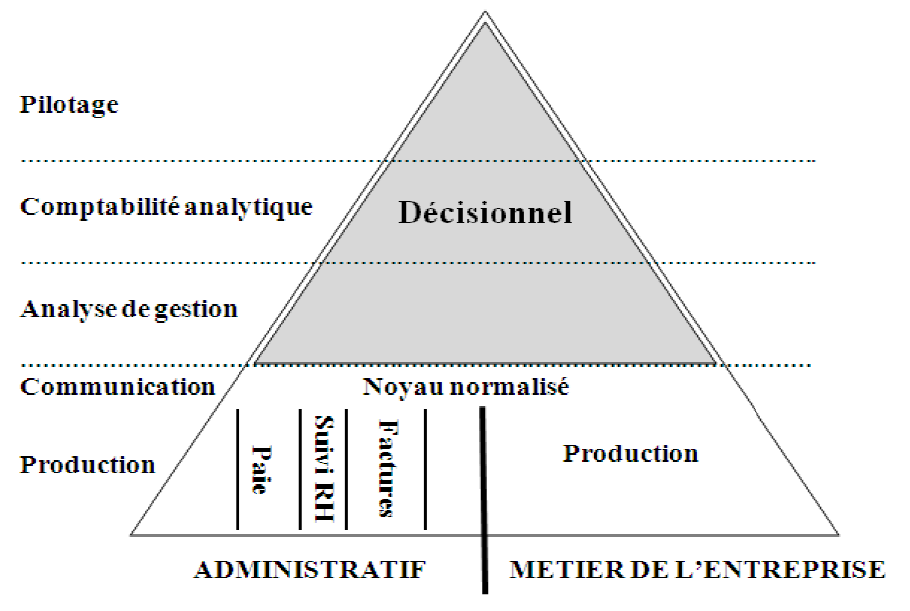
\includegraphics[width=\textwidth]{decisionnelauseindusi}
    \caption{Le décisionnel au sein du Système d’information}
    \label{fig:decisionnelauseindusi}
\end{figure}

\subsection{Différents composantes du décisionnel}
En relation étroite avec les nouvelles technologies de l’information et des télécommunications, le système décisionnel se manifeste à différents niveaux selon leurs utilités et leurs missions principales, comme illustré dans la figure \ref{fig:composantsdudecisionnel} [Goglin, 1998].

\begin{figure}[H]
    \centering
    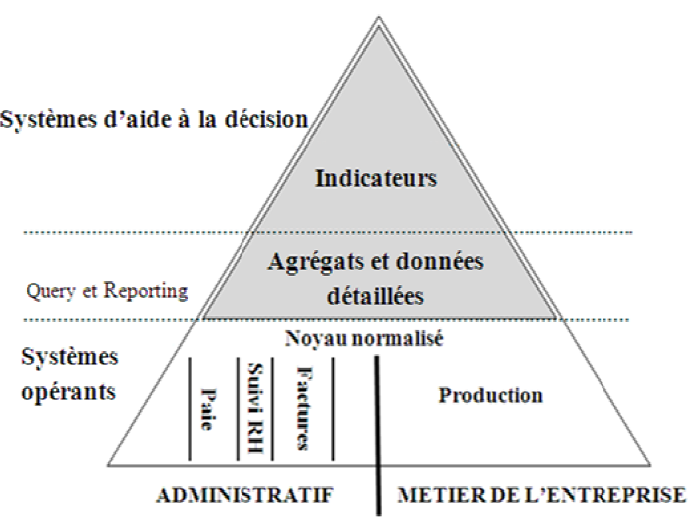
\includegraphics[width=\textwidth]{composantsdudecisionnel}
    \caption{Les différentes composantes du décisionnel}
    \label{fig:composantsdudecisionnel}
\end{figure}

\subsection{Décisionnel vs transactionnel}
Le système transactionnel permet de gérer les données en production en temps réel. Il est conçu pour l’insertion, la modification, interroger rapidement, efficacement et en sécurité les données de la base, sélectionner, ajouter, mettre à jour, supprimer des tuples et répondre à de nombreux utilisateurs simultanément.
\paragraph{}
Mais il y a des requêtes complexes et lourdes qui abîment les performances des systèmes transactionnels, et des données temporelles réparties rendent la vue historique de données difficile. Le système décisionnel gère les données agrégées, calculées selon des axes (critères d’analyse) prédéterminés à des fins d’analyse.
\paragraph{}
Le tableau \ref{tab:comparatifdecisonneltransactionnel} résume de façon non exhaustive les différences qu’il peut y avoir entre les systèmes transactionnels et les systèmes décisionnels selon les données et l’usage fait des systèmes.

\begin{table}[H]
    \centering
    \caption{Comparaison des systèmes transactionnels et les systèmes décisionnels.}
    \begin{tabular}[t]{|p{3cm}|p{6cm}|p{6cm}|} 
        \hline
        \textbf{Différence} & \textbf{Systèmes transactionnels} & \textbf{Systèmes décisionnels} \\
        \hline\hline
        \multirow{5}{5em}{Par les données} & Orienté applications & Orienté thèmes et sujets \\
        & Situation instantanée & Situation historique \\ 
        & Donnée détaillées et codées non redondantes & Informations agrégées cohérentes souvent avec redondance \\ 
        & Données changeantes constamment & Informations stables et synchronisées dans le temps \\ 
        & Pas de référentiel commun & Un référentiel unique \\ 
        \hline
        \multirow{5}{5em}{L’usage} & Assure l’activité au quotidien & Permet l’analyse et la prise de décision \\
        & Pour les opérationnels & Pour les décideurs \\ 
        & Mises à jour et requêtes simples & Lecture unique et requêtes complexes
        transparentes \\ 
        & Temps de réponse immédiats & Temps de réponse moins critiques \\ 
        & Faibles volumes à chaque transaction & Large volume manipulé \\ 
        & Conçu pour la mise à jour & Conçue pour l’extraction \\ 
        & Usage maîtrisé & Usage aléatoire \\ 
        \hline\hline
    \end{tabular}
    \label{tab:comparatifdecisonneltransactionnel}
\end{table}%


\section{Les entrepôts de données ou « Datawarehouse »}

Les entrepôts de données sont apparus en 1996, réponse au besoin de rassembler toutes les informations d’une entreprise en une base de données unique destinée aux analystes et aux gestionnaires. Celà en intègrant des informations provenant de différentes sources de données internes mais aussi externes à l’environnement de l’organisme et en offrant la possibilité de faire des analyses et des corréllations sur des agrégations crééés dynamiquement à partir de plusieurs dimentions.
\paragraph{}
Les bases de données des systèmes existants de type OLTP\footnote{Online Transaction Processing} ne sont pas appropriées comme support d’analyse, vu que leur conception ne vise pas les fonctions spécifiques réalisées dans l’entreprise. D’où la nécessité de la mise en place d’un système décisionnel qui fournit une vue globale des informations de l’entreprise et aussi un moyen stratégique de prise de décision.

\subsection{Notion de Datawarehouse}
Bill Inmon définit l’entrepôt de données dans son ouvrage "Building Data warehouse" de la façon suivante : L’entrepôt de données est une collection de données orientées sujet, intégrées, non volatiles et historiées, organisées pour support d’un processus d’aide à la décision".
\paragraph{}
Cette définition d’ED\footnote{Entrepôt de Données} a été conceptualisée en termes de caractéristiques du référentiel des données, qui seront détaillées dans les points suivants :

\begin{itemize}
    \item \textbf{Orientées sujet :} Les données de l’entrepôt sont organisées par thème (autour des sujets majeurs et des métiers de l’entreprise). L’intérêt dans cette organisation est de disposer d’un ensemble d’informations utiles sur un sujet transversal aux structures fonctionnelles et organisationnelles de l’entreprise. \cite{book:5}
    \item \textbf{Intégrées :} Les données dans l’entrepôt proviennent de différentes sources éventuellement hétérogènes. L’intégration est un processus qui consiste à résoudre les problèmes d’hétérogénéité, où les données contenues dans ED sont divisées en grandes subdivisions appelées domaine. \cite{book:6}
    \item \textbf{Non volatiles :} Les données stockées au sien de l’entrepôt sont permanentes et ne peuvent être modifiées, et le rafraîchissement de l’entrepôt de données, consiste seulement à ajouter de nouvelles données sans modifier ou perdre celle qui existent. Ceci pour conserver la traçabilité des informations et des décisions prises. \cite{book:6}
    
    \begin{figure}[H]
        \centering
        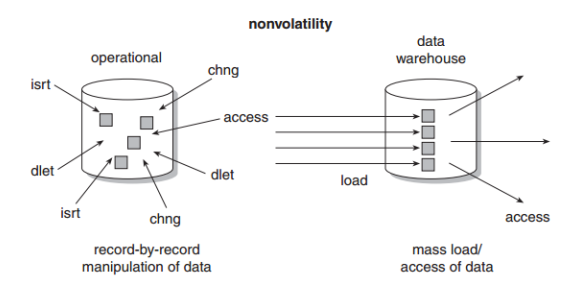
\includegraphics{nonvolatilitedonnees}
        \caption{Non volatilité des données de l’ED.}
        \label{fig:composantsdudecisionnel}
    \end{figure}

    La figure \ref{fig:composantsdudecisionnel} extrait de l'ouvrage de William Ilmon 'Building the Datawarehouse' \cite{book:7} démontre la non volatilité des données dans les entrepôt de données.

    \item \textbf{Historisées :} Pour suivre dans le temps l’évolution des différentes valeurs des indicateurs à analyser, l’historisation est nécessaire. Un référentiel de temps est associé aux données, afin de permettre l’identification dans la durée de valeurs précise. \cite{book:5}
\end{itemize}


\subsection{Historique des Datawarehouses}
L’origine des ED revient à 1960, ou l’entreprise General Mills et l’Université Dartmouth, dans un projet conjoint, créent les termes "faits" et "dimensions".Les dates marquantes de l’histoire des entrepôts de données sont : \cite{book:8}
\begin{itemize}
    \item En \textbf{1983}, Teradata introduit dans son SGBD un système purement décisionnel.
    \item En \textbf{1988}, Le terme DataWarehouse est utilisé pour la premiere fois dans l’article "An architecture for business and information systems" publier par Barry Devlin et Paul Murphy dans le journal système d’IBM.
    \item En \textbf{1990}, Red Brick Systems construit le système "Red Brick Warehouse" dédié à la construction d’entrepôt de données.
    \item En \textbf{1991}, Bill Inmon publie le livre "Building the Data warehouse".
    \item En \textbf{1995}, La création de l’organisation "Data Warehousing Institute" pour soutenir et promouvoir la recherche dans le domaine des ED.
    \item En \textbf{1996}, Ralph Kimball publie le livre "The Data Warehouse Toolkit".
    \item En \textbf{1997}, Réalisation de "Oracle 8", avec la prise en charge des requêtes des schémas
    en étoiles.
\end{itemize}

% \subsubsection{Eléments d’un Datawarehouse}
% \blindtext

\subsection{Différence entre Datawarehouse et base de données}
Le concept d’un entrepôt de données est apparu lors de l’existence de différence entre les systèmes transactionnels en ligne (OLTP) et les systèmes informationnels, dont certaines de ces différences fondamentales sont listées à travers le Tab1.1.Mais d’autres méthodes et techniques de conception et d’implémentation d’ED ont vu le jour, l’une de ces techniques est le modèle dimensionnel de Kim Bail apparue en 1996. \cite{thesis:1}

\begin{table}[H]
    \centering
    \caption{Comparaison entre les bases de données et les entrepôts de données.}
    \begin{tabular}[t]{|p{3cm}|p{6cm}|p{6cm}|} 
        \hline
        \textbf{Foncionnalités} & \textbf{Base de données} & \textbf{Entrepôt de données} \\
        \hline\hline
        Caractéristiques & Basé sur le traitement optionnel & Basé sur le traitement
        d’information \\
        \hline
        Données & Actualisation de données stockées & Historisation de données stockées \\ 
        \hline
        Fonction & Les opérations quotidiennes & Les besoins d’information à long terme et aide à la décision \\ 
        \hline
        Utilisateur & Employés & Analystes, décideurs \\ 
        \hline
        Unité de travail & Court et simple transaction & Requêtes complexes \\ 
        \hline
        Orientation & L’orientation est sur la transaction & L’orientation est sur l’analyse \\ 
        \hline
        Vue & La vue des données est relationnelle plate & La vue des données est multidimentionnelle \\ 
        \hline
        Accès & Lecture et écriture & Lecture et rafraîchissement \\
        \hline
        Taille & Plusieurs gigaoctets & Plusieurs teraoctets \\
        \hline
        Priorité & Haute performance, haute disponibilité & Grande flexibilité, l’autonomie de l’utilisateur final \\
        \hline
        Métrique & Mesurer l’efficacité le débit, le débit transactionnel & Mesurer l’efficacité, le débit de la requête et le temps de réponse \\ 
        \hline\hline
    \end{tabular}
    \label{tab:comparaisonbdded}
\end{table}%



\section{Les processus ETL}
« Extract-Transform-Load » est connu sous le terme ETL (ou parfois : datapumping). Il s'agit d'une technologie informatique intergicielle (comprendre middleware)\footnote{Un logiciel tiers qui crée un réseau d'échange d'informations entre différentes applications informatiques.} permettant d'effectuer des synchronisations massives d'information d'une base de données vers une autre. Selon le contexte, on traduira par « extraction », « transformation », « alimentation ». La figure \ref{fig:etl} extrait du site web officiel de SupINFO \cite{website:1}, démontre le travail du processus ETL. 

\begin{figure}[H]
    \centering
    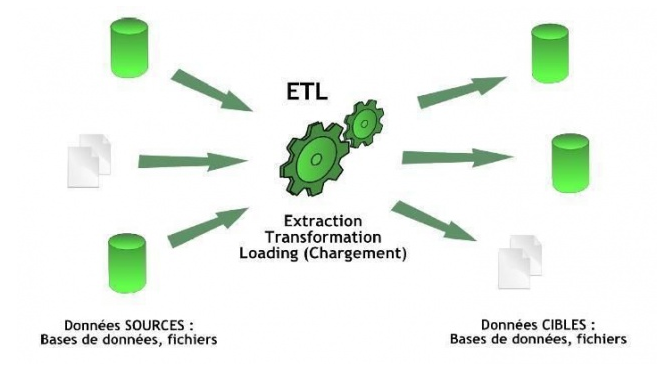
\includegraphics{etl}
    \caption{Extraction - Transformation - Chargement}
    \label{fig:etl}
\end{figure}

\subsection{Notion d’ETL}
L'ETL représente la zone de construction qui contient l’ensemble d’outils et techniques utilisés lors du processus de préparation des données, avant leurs chargements au niveau de l’entrepôt, qui sont utilisés pour alimenter les bases de données opérationnelles qui se situent au niveau du Data warehouse tier. Comme son nom l’indique, l’ETL est un processus à trois étapes.

\subsection{Extraction des données}
Consiste à recueillir des données hétérogènes provenant de multiples sources, base de données opérationnelles, ou des fichiers de différents formats ; ils peuvent être des sources internes à l’organisation ou extérieures. Pour résoudre les problèmes d’interopérabilité, les données sont extraites chaque fois que possible en utilisant l’interface du programme d’application, telles que ODBC (Open DataBase Connection), OLEDB (Open Linking and Embedding for DataBase) et JDBC (Java DataBase Connectivity). \cite{book:10}

\subsection{Transformation des données}
Une fois que les données sont extraites du système source, elles subissent une série de traitements destinée à les transformer en informations présentables.Cette procédure comporte plusieurs aspects : \cite{book:11}
\begin{itemize}
    \item le nettoyage, ce qui supprime les erreurs et les incohérences dans les données et les convertit en un format normalisé ; 
    \item l’intégration, qui concilie les données provenant de différentes sources de données, au niveau schéma et données ; 
    \item et l’agrégation, qui résume les données obtenues à partir de sources de données en fonction du niveau de détail, ou la granularité, de l’entrepôt de données.
\end{itemize}

\subsection{Chargement des données}
Alimente l’entrepôt de données avec les données transformées en respectant les contraintes du SGBD cible. Cela inclut également le rafraîchissement de l’entrepôt de données à savoir, la propagation des mises à jour dans l’entrepôt de données à partir des sources de données à une fréquence spécifiée afin de fournir des données à jour pour le processus de prise de décision. \cite{book:10}

\paragraph{}
Le processus ETL nécessite généralement une zone de préparation de données (data staging). Le data staging représente le chantier de l’ED. C’est là que les données sont chargées, nettoyées, combinées, archivées, puis rapidement exportées vers l’entrepôt. L’objectif de cette zone est l’obtention de données prêtes à être chargées sur un serveur de présentation (un moteur OLAP ou un SGBDR) \cite{book:12}



\section{Les magasins de données ou « datamarts »}
Un Datamart est un sous élément du DataWarehouse , également sous le nom de « magasin de données » ou « comptoir de données » Outil aux prémices du Big Data, son but n’est pas de rassembler des données avant de les trier mais au contraire de les organiser selon des usages métiers ou des domaines ciblés. En effet, sous-ensemble du DataWarehouse, il contient des informations se rapportant à un secteur d'activité particulier de l'entreprise ou à un métier qui y est exercé. Ils servent à des utilisateurs dans l’entreprise et répondent à leurs besoins ; on parle notamment de Datamart financier, de Datamart marketing, de Datamart commercial…
\paragraph{}
Au sein d’une entreprise, les différents services de celle ci auront besoin chacun de données qui leurs seront propres. Le Datamart a justement été crée pour regrouper au sein d’une base ces informations propres à un service ou plus généralement à une fonction. De ce fait, à une fonction correspond un Datamart. Les bases de données pourront être traitées et préparées plus finement, de manière plus orientée et avec une grande précision.
\paragraph{}
Le Datamart rassemble un ensemble de données regroupées, organisées, agrégées et ciblées dans le seul et unique but de répondre aux besoins des métiers. Au sens technique, il est créé à partir d’une base de données relationnelle exploitée à partir du langage informatique SQL\footnote{Structured Query Language, pour les requêtes sur les bases de données} et stockée physiquement sur un disque dur par le biais d’un système de gestion de base de données. Il se situe en aval du DataWarehouse et est alimenté par celui-ci. Les notions que nous venons de decouvrir ainsi que la figure \ref{fig:datamart}, qui démontre la relation entre le Datamart et le Datawarehouse ont étés extraites d'une page web parlant des Datamarts et des Datawarehouse sur le site officiel de SupINFO \cite{WEBSITE:2}
\begin{figure}[H]
    \centering
    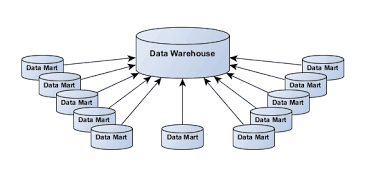
\includegraphics{datamart}
    \caption{Ensemble de Datamarts formant un Datawarehouse}
    \label{fig:datamart}
\end{figure}


\section{Les cubes OLAP}

\subsection{Concept OLAP}
Le terme OLAP (On-Line Analytical Processing) désigne une classe de technologies conçue pour l’accès aux données et pour une analyse instantanée de ces dernières, dans le but de répondre aux besoins de Reporting et d’analyse.
\paragraph{}
R. Kimball définit le concept « OLAP » comme \textit{« Activité globale de requêtage et de
présentation de données textuelles et numériques contenues dans l’entrepôt de données; Style
d’interrogation spécifiquement dimensionnel » }. \cite{book:14}

C’est en continuant sur sa lancée, qui lui a permis de définir le model OLTP pour les bases de données relationnelles, que le concept OLAP fut introduit et défini6 en 1993 par E.F Codd, le père des bases de données relationnelles, dans un document technique portant le titre de « Providing OLAP (On-Line Analytical Processing) to User-Analysts : An IT Mandate ». \cite{ARTICLE:1}

\subsection{Notion de cube}
D'après Mahèzi Magnouwai dans un article \textit{"Cube OLAP, rapports basés sur un cube"} \cite{WEBSITE:6}, un cube OLAP est une base de données à plusieurs dimensions optimisées pour réaliser des applications décisionnelles. Le cube est un outil d’analyse multidimensionnelle destiné aux utilisateurs métier. La figure \ref{fig:olapcube} provient du même article.

\begin{figure}[H]
    \centering
    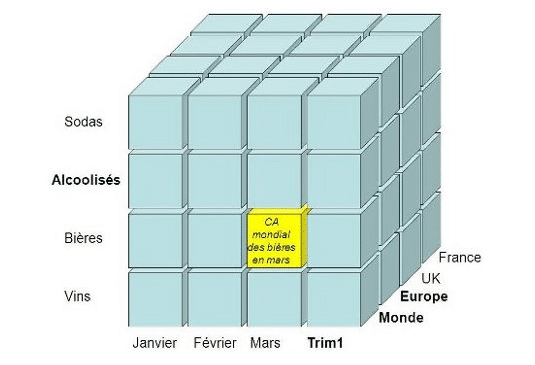
\includegraphics{olapcube}
    \caption{Représentation conceptuel d'un cube OLAP}
    \label{fig:olapcube}
\end{figure}

\paragraph{}
Elle continue en disant que dans les cubes OLAP, les données sont classées par dimension. Les cubes sont pré-synthétisés entre les dimensions et les données sont agrégées afin d’accélérer considérablement l’interrogation par rapport aux bases de données relationnelles. Le cube étant aussi considéré comme une base de données, elle stocke les informations comme le ferait une base de données traditionnelle mais sa structure est différente. Historiquement, les bases de données sont conçues selon les exigences des systèmes informatiques qui les utilisent. En revanche, les cubes OLAP sont exploités par des utilisateurs métiers en vue de faire des analyses. Le cube sert aussi d’une couche entre l’entrepôt de données (datawarehouse) et l’utilisateur final. Un cube OLAP a les caractéristiques suivantes :
\begin{itemize}
    \item il permet d’obtenir des informations déjà agrégées selon les besoins de l’utilisateur. Pas besoin de créer donc un rapport pour chaque besoin de l’utilisateur;
    \item il est simple à utiliser avec des mécanismes de « drag and drop ». Vous n’avez juste qu’à faire des glisser-déposer des données que vous souhaitez analyser. Les cubes sont rapides daccès. Généralement le cube ne contient pas toutes les données de l’entrepôt de données;
    \item il permet d'avoir la possibilité de manipuler des données agrégées selon différentes dimensions (axes);
    \item un cube utilise les fonctions classiques d’agrégation : min, max, count, sum, avg, mais peut également utiliser des fonctions d’agrégations spécifiques.
\end{itemize}
\paragraph{}
Tout comme les bases de données qui ont un langage qui permet de les gerer : le langage est SQL (Structured Query Language) mentionne un peu plus haut, les cubes OLAP disposent également d’un langage appelé le langage MDX (Multidimensional Expression).


\subsection{Langage de navigation : « MDX »}
Le MDX (de l'anglais Multidimensional Expressions, « expressions multidimensionnelles ») est un langage de requête pour les bases de données OLAP, analogue au rôle de SQL pour les bases de données relationnelles. C'est aussi un langage de calcul avec une syntaxe similaire à celle des tableurs.
\paragraph{}
Le langage des expressions multidimensionnelles possède une syntaxe appropriée à l'interrogation et manipulation des données multidimensionnelles mémorisées dans un cube OLAP. Bien qu'il soit possible de traduire certaines expressions dans le langage SQL traditionnel, cela nécessite une syntaxe SQL souvent maladroite même pour des expressions MDX très simples. MDX a été adopté par une large majorité de fournisseur de la technologie OLAP et est devenu un standard de facto pour les systèmes OLAP.


\section{Les systèmes de « reporting »}
Le terme "Reporting" désigne une famille d'outils de Business intelligence destinés à assurer la réalisation, la publication et la diffusion de rapports d'activité selon un format prédéterminé. Ils sont essentiellement destinés à faciliter la communication de résultats chiffrés ou d'un suivi d'avancement.

\subsection{Notion de reporting}
Alain Fernandez dans son article intitulé \textit{"La création et la publication de rapport d'activité"} \cite{WEBSITE:4} nous fait savoir que l'outil de reporting assure l'interrogation des bases de données selon les requêtes SQL préparées lors de l'élaboration du modèle. Le rapport d'activité peut ensuite être publié sur l'Intranet, périodiquement en automatique ou ponctuellement à la demande. L'outil offre bien entendu des fonctions spécifiques pour l'élaboration du modèle du rapport, des modules de calcul et de présentation (graphiques) afin de concevoir des comptes rendus particulièrement seyants et pertinents.
\paragraph{}
Il continue en disant qu'avec les outils requêteurs, l'utilisateur peut formuler des requêtes d'interrogation "ad hoc" à volonté. Les outils de reporting ne sont pas à proprement parlé des instruments d'aide à la décision. Bien que, lorsqu'ils sont utilisés correctement, on peut juger qu'ils permettent au responsable de disposer d'une précieuse vue d'ensemble de son activité, ils sont en fait surtout destinés à "rendre compte" du travail effectué auprès de la hiérarchie. 
\paragraph{}
Le reporting s'inscrit dans une longue tradition du management par le contrôle. Nous sommes bien loin des possibilités d'autonomie que peut offrir la technologie de la Business Intelligence aujourd'hui.

\begin{figure}[H]
    \centering
    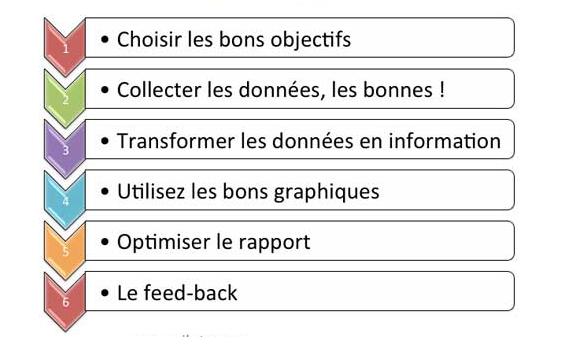
\includegraphics{reportingreussi}
    \caption{Un reporting réussi}
    \label{fig:reportingreussi}
\end{figure}

Provenant du même article, la figure \ref{fig:reportingreussi} montre les étapes à suivre pour obtenir un "rapport réussi". Un "rapport réussi" est un rapport suffisamment pertinent et correctement présenté pour intéresser ses destinataires, soutenir l'attention et susciter des commentaires constructifs.

\subsection{Analyse ad-hoc}
Margaret Rouse dans son article \textit{"Analyse ad hoc"} sur LeMagIT \cite{WEBSITE:5} a ecrit les paragraphes suivants sur l'analyse ad hoc.
\paragraph{}
L'analyse ad hoc est un processus d'informatique décisionnelle (BI) conçu pour répondre à une question métier unique et précise. Le résultat d'une analyse ad hoc est généralement un modèle statistique, un rapport analytique ou une forme quelconque de synthèse des données. 
\paragraph{}
Selon le Larousse, ad hoc « se dit d'une règle, d'un raisonnement élaborés uniquement pour rendre compte du phénomène qu'ils décrivent, ne permettant donc aucune généralisation ». Une analyse ad hoc a pour objet de combler les lacunes laissées par les rapports réguliers, mais statiques de l'entreprise. Elle peut servir à créer un rapport qui n'existe pas encore ou à approfondir un rapport statique pour obtenir des détails sur des comptes, transactions ou enregistrements. Le processus permet également de recueillir des données plus récentes dans les domaines déjà couverts par un rapport statique.
\paragraph{}
Les tableaux de bord OLAP sont spécialement conçus pour faciliter l'analyse ad hoc en offrant un accès rapide et facile aux données du rapport d'origine. En effet, si l'utilisateur (généralement un responsable ou un cadre) peut accéder lui-même aux données par une interface de type « point-and-click », il devient inutile de demander une analyse à une autre entité de l'entreprise. Ainsi, cette fonctionnalité accélère les temps de réponse lorsqu'une question métier se présente, ce qui permet à l'utilisateur de réagir et de prendre ses décisions plus rapidement.
\paragraph{}
Bien que destinés à un usage unique, la plupart des rapports et analyses ad hoc finissent souvent par être réutilisés et exécutés régulièrement. Cette pratique relativement courante peut conduire à des processus superflus, qui se révèlent particulièrement lourds dans les périodes de reporting intense. Par conséquent, il convient de revoir périodiquement les rapports en fonction de critères d'efficacité, afin de déterminer s'ils sont toujours utiles.

\subsection{Reporting de masse}
Tiré du livre blanc de Anne-Marie Abisségué intitulé \textit{"Le reporting de masse : état des lieux et nouveaux enjeux"} \cite{book:13}, le reporting de masse désigne les outils reposant sur des techniques d'interrogation, de reporting et de diffusion automatisées d'une information personnalisée vers un grand nombre d'utilisateurs. L'évolution des systèmes décisionnels en entreprise est poussée par la nécessité de mettre à disposition du plus grand nombre d’employés des outils d’accessibilité à l’information adaptés leurs besoins. L'objectif étant d'avoir une masse d’information pour prendre les bonnes décisions et mettre en place les bonnes actions.
\paragraph{}
A cette étape du développement des systèmes décisionnels, ce sont davantage les capacités de découverte et d'analyse de l'information des outils qui ont été mises en avant. Mais l'utilisation de ces outils présente des contraintes aussi bien en terme de rapidité d'exécution de la requête demandée (plusieurs heures, voire plusieurs jours), qu'en terme de compétence nécessaire pour les manipuler (ces outils mobilisent des analystes spécialisés). Les limites des outils décisionnels traditionnels sont vite atteintes, car leur utilisation reste le fait d'un nombre restreint d'utilisateurs.

\begin{figure}[H]
    \centering
    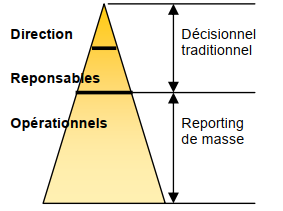
\includegraphics{reportingmasse}
    \caption{La place du reporting de masse}
    \label{fig:reportingmasse}
\end{figure}
 Provenant du même livre que les paragraphes précédentes, la figure \ref{fig:reportingmasse} montre la place du reporting de masse dans l'entreprise. La connaissance et l'analyse de l'information par un petit cercle de personnes dans l'entreprise ne suffisent plus. L'information doit être accessible au plus grand nombre dans l'entreprise, une nécessité imposée par les nouveaux contextes organisationnels.



% \subsection{Les systèmes de visualisation de données}

% \subsubsection{Notion de visualisation des données}
% \blindtext

% \subsubsection{Historique de la visualisation des données}
% \blindtext

% \subsubsection{Fonctions de la visualisation des données}
% \blindtext



\section{Gestion commerciale et décisionnel}
L’entreprise, qu’elle soit multinationale ou une TPE\footnote{Très Petite Entreprise}, doit vendre pour « survivre ». C’est aussi sa vraie mission : la rentabilité ! Pour assurer cette mission, l’aspect commercial est très important. Dans un contexte aussi concurrentiel, l’entreprise ne peut plus se contenter de « vendre » mais doit planifier une vraie stratégie commerciale qui se traduira dans sa gestion commerciale. C’est pourquoi la gestion commerciale est l’un des piliers d’une entreprise qui réussit.
\paragraph{}
La gestion commerciale s’occupe de toute la chaîne nécessaire à la production de biens/services en vue de leur vente. Elle va donc prendre en charge la prévision, la réalisation et le suivi des ventes. La gestion commerciale englobe aussi bien la fonction achat, que la logistique ou encore la facturation et la vente (dont celle de l’après-vente). 

\subsection{Importance de la gestion commerciale}
Marion, en 2017 \cite{WEBSITE:3} dans son article \textit{"L’importance de la gestion commerciale en entreprise"} dit que pour trouver la bonne solution gestion commerciale, il convient d’en comprendre la notion. Cette procédure englobe tous les besoins liés à la production des biens ou services pour la vente. Cette gestion prend ainsi en charge de la prévision, de la réalisation et du suivi des ventes. Elle réunit également la fonction d’achat, la logistique ou encore la facturation et l’après-vente. À titre de rappel, une bonne gestion commerciale assure le pilotage de l’entreprise. C’est la gestion commerciale qui s’occupe de fixer les prix de vente des services ou des produits, effectuer le suivi des stocks ou encore la gestion des relations clients ainsi que la gestion des relations avec les fournisseurs. On entend par là les relances des créances impayées. C’est également en se basant sur les données du département commercial que les dirigeants pourront prendre des décisions stratégiques. 

\subsection{Objectifs des outils de gestion commerciale}
Facturation, suivi de livraison, relances client… La gestion commerciale est un service clé de l’entreprise. Elle est facilitée par des outils de gestion informatique de plus en plus efficaces.

L'objectif principal de la gestion commerciale est de réaliser, prévoir et développer la vente des biens ou des services. Les fonctions commerciales sont présentes aussi bien dans le B to B (business to business, qui désigne la vente aux entreprises) que dans le B to C (business to consumer, qui signifie « vente au grand public »).

Elle est prévue pour optimiser la chaîne de valeur des entreprises (ensemble d'activités interdépendantes visant à générer de la valeur) en regroupant les processus internes.

La gestion commerciale s’occupe de toute la chaîne nécessaire à la production de biens et services. Ses missions principales sont :
\begin{itemize}
    \item la conquête de nouveaux clients ;
    \item le développement de clients et de projets ;
    \item le développement d’activités à l’international ;
    \item le développement de partenariats stratégiques, afin de préparer la croissance future.
\end{itemize}
La gestion commerciale fournit également les indicateurs de marché permettant aux dirigeants de réaliser les choix stratégiques pertinents.

\subsection{Fonctions des outils de gestion commerciale}
Selon l’Association pour l'Emploi des Cadres (APEC)\footnote{https://recherche-d-emploi.ooreka.fr/comprendre/apec}, la gestion commerciale recrute plus de 30 000 cadres par an. En pratique, cette filière s’articule autour des fonctions suivantes :
\begin{itemize}
    \item achat et relations avec les fournisseurs ;
    \item fixation des prix de vente ;
    \item prévision, réalisation, relations, suivi des stocks ;
    \item vente, facturation, fidélisation et relances clients ;
    \item contrôle de gestion commerciale.
\end{itemize}
\paragraph{}
Dans le détail, les logiciels de gestion commerciale, de dernière génération permettent :
\begin{itemize}
    \item la création de devis, factures et bons de livraison ;
    \item la gestion des comptes et commandes client ;
    \item le suivi des achats et des ventes ;
    \item le transfert des données en comptabilité ;
    \item l’édition des les relevés des clients en attente de paiement ou de facturation (balance âgée) ;la gestion des stocks en temps réels ;
    \item la gestion des commerciaux.
\end{itemize}




 



\section*{Conclusion}%
\addcontentsline{toc}{section}{\numberline{}Conclusion}%
%Le but de ce chapitre étant de faire une revue de littérature, sortir la problématique, étudier l’existant et proposer une solution, nous en ressortons que l’entreprise a besoin d’une plateforme de Business Intelligence pour pallier a ses problèmes de fixation des prix et comment savoir quels produits seront demandés pour des périodes spécifiques.
Le but de ce chapitre étant de faire une revue de littérature pour présenter les concepts qui seront abordés dans ce projet, nous avons fait le tour des notions et concepts et nous sommes à présent armés de connaissances qui nous seront utiles pour la suite du projet.


\newpage
\chapter{Cahier de Charges et Analyse}

\section*{Introduction}%
\addcontentsline{toc}{section}{\numberline{}Introduction}%
Comme son nom ce chapitre a pour but de ressortir les différents éléments présents dans le cahier de charges d’un projet. Nous allons commencer par étudier la problématique dont fait face l’entreprise et de là nous allons faire une étude de l’existant. Le résultat de ceci nous guidera dans le choix d’une solution que nous allons présenter, puis nous allons analyser la solution pour en ressortir les fonctionnalités. De là nous seront en mesure de faire une planification pour notre projet ainsi qu’une estimation des couts.
\section{Problématique}
\subsection{Présentation du cas d’études : AMD Sarl}
AMD est l'agent / distributeur exclusif au Cameroun de plusieurs categories de materiaux de maintenance industrielle. De ce fait la gestion commerciale est un element cle dans la survie economique de l'entreprise. AMD Sarl est une PME et comme la plupart des entreprises, pour leur aider dans la gestion de leurs activités au quotidien y compris la gestion commerciale, ils utilisent un outil de gestion commerciale en ligne, notamment l’ERP\footnote{Enterprise Resource Planning (Progiciel de Gestion Intégré en français)} Sage 100.
Cependant l'entreprise a souvent besoin d'optimiser le processus de fixation des prix de leurs produits ou encore savoir a quel moment avoir un certain produit en stock, ce qui pourrait nettement améliorer les ventes de l'entreprise. Ceci est rarement optimal. De ce fait ca devient plus difficile pour l'entreprise de fidéliser les clients ou encore acquérir des nouveaux clients. 
\subsection{Démarche d’analyse du problème}
Pour mieux analyser notre problème, on a résolu à utiliser la méthode des 5M. Aussi appelé diagramme de causes/effets" ou "en arêtes de poisson", l'outil créé par Mr Ishikawa fait partie de ceux à posséder dans sa trousse à outils spéciale "résolution des problèmes". Rappelant le squelette d'un poisson, cet outil visuel a pour finalité de lister les causes qui ont une influence sur un effet (une situation), de les classer, de les hiérarchiser. Très utilisé par les qualiticiens, le diagramme d'Ishikawa est en fait applicable à l'ensemble des métiers de l'entreprise.
\paragraph{}
Les étapes principales dans l’utilisation de cette méthode sont les suivants :
\begin{itemize}
    \item \textbf{Qualifiez l'effet :} Il s'agit couramment du problème que vous cherchez à résoudre. Dans notre contexte on peut identifier les effets suivants :
    \begin{itemize}
        \item La diffculté à fixer un prix pouvant generer un gain maximal à un moment précis
        \item Savoir a quel moment avoir un produit en particulier en stock et la quantité pour éviter des clients insatisfaits.
    \end{itemize}
    \item \textbf{Dressez un inventaire des causes possibles }: Il s’agit de lister les causes qui ont une influence sur le problème. Dans notre contexte on peut constater que l'entreprise possède des données généres par ses systèmes de gestion qui ne sont pas exploitées. De ce fait il ya un maque d'outils pouvant aider à faire des décisions.
    \item \textbf{Classez les causes par familles :} Ici intervient les 5M qui sont fréquemment utilisés pour cette tâche : Main d’œuvre, matière, matériels, méthodes, milieu. Dans notre cas on a une seule catégorie qui est la méthode d'utilisation de nos données.
    \item \textbf{Evaluez les branches/racines qui ont le plus d'impact.}
\end{itemize}

Le diagramme Ishikawa dans la figure \ref{fig:ishikawa} nous montre l'origine des problématiques dont fait face l'entreprise.
\begin{figure}[H]
    \centering
    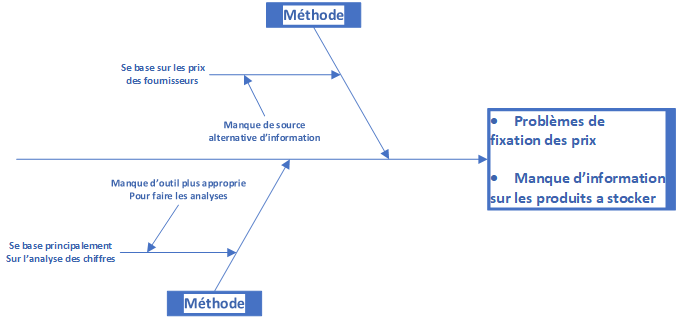
\includegraphics[width=\textwidth]{ishikawa}
    \caption{Diagramme Ishikawa analysant nos problématiques}
    \label{fig:ishikawa}
\end{figure}


\subsection{Identification de la problématique}
L’entreprise possède une quantité énorme d’informations non exploités, qui peuvent non seulement optimiser la prise de décisions par les décideurs mais aussi faciliter le travail des employés, augmentant ainsi la productivité de celles-ci, si exploitée de la bonne façon. 

De ce fait on peut identifier les problématiques suivantes, aussi représentés dans la figure 
\begin{itemize}
    \item La difficulté à fixer le prix d'un produit pour avoir un revenue maximal sur celui ci dans période bien précise.
    \item La difficulté dans l'identification des produits à mettre en stock avec les quantités à une certaine période pour éviter d'avoir des clients qui commandent des produits qu'on ne peut pas fournir.
\end{itemize}



\section{Etude de l’existant}
Nous ne saurions débuter ce travail sans avoir une idée claire et précise sur l’existant quel qu’il soit. La première tâche a été de rencontrer les différentes personnes qui sont ou peuvent être impliquées dans les prises de décision et la gestion commerciale en général dans l’entreprise. 
\paragraph{}
Nous avons principalement travaillé avec le chef du département de l’approvisionnement, de la recherche et de l’innovation, M. Arnold KOGAING. Après quoi, nous avons réellement débuté le travail en menant différentes recherches. Cette méthodologie de travail nous a permis d’avoir une connaissance large de l’existant.

\subsection{La gestion commerciale à AMD}
AMD Sarl est une PME et comme la plupart des entreprises, pour leur aider dans la gestion de leurs activités au quotidien y compris la gestion commerciale, utilisent un outil de gestion commerciale en ligne, notamment l’ERP Sage 100.
\paragraph{}
Sage 100 est un logiciel qui propose d’accompagner les petites et moyennes entreprises dans la gestion de leurs ressources. De la gestion commerciale en passant par la comptabilité et les fonctionnalités de pilotage, Sage 100 s’impose comme un outil indispensable aux PME. Pour autant, la gestion des clients tout comme celle des achats et des fournisseurs ne sont pas en reste puisque Sage 100 propose une gestion puissante du cycle de vente du début de la chaîne jusqu’à sa fin.
\paragraph{}
Sage 100 est assez récent dans l’entreprise avec d’autres outils tels Gescom v14 et MS Excel utilisés pour gérer les processus de gestion commerciale. 

\subsubsection{Outils de gestion commerciale}
Le tableau \ref{tab:outilsdegescom} decrit un peu l'historique des outils des gestion commerciale utilisés par AMD.

\begin{table}[H]
    \centering
    \caption{Tableau des outils de gestion commerciale utilisés au fil du temps.}
    \begin{tabular}[t]{|p{3cm}|p{7cm}|p{5cm}|} 
        \hline
        \textbf{Outil} & \textbf{Description} & \textbf{Période} \\
        \hline\hline
        Sage 100 & ERP offrant de nombreuses fonctionnalitées & Moins de 10 mois d'utilisation \\
        \hline
        Gescom v14 & ERP, offrant moins de fonctionnalites que Sage 100 et les données sont moins descriptifs. Données pas aussi  fiables que celles de Sage 100  & Utilisation sur 3 années avant Sage 100 \\ 
        \hline
        Microsoft Excel & Tableur, permettant de concevoir de modèle de gestion assez complexes. Données encore moins fiables que celles de Gescom v14 & Utilisation sur 10 ans avant Gescom v14 \\ 
        \hline
        Traces papiers & Utilisation de papiers pour garder toute traces des transactions effectués par l’entreprise. & Dès la création de l’entreprise jusqu’à l’introduction de MS Excel. \\ 
        \hline\hline
    \end{tabular}
    \label{tab:outilsdegescom}
\end{table}%

\subsubsection{Prises de décisions en gestion commerciale}
Concernant de départements en entier, les décisions finales sont prises par le directeur général de l’entreprise après une ou plusieurs réunions avec les responsables dans le département en question et d’autres cadres. Ces réunions incluent souvent des brainstormings ou encore des analyses des chiffres. Il peut aussi arriver que le directeur se fie à son intuition pour prendre une décision. La figure \ref{fig:niveaudeladecision}, extraite d'un document en ligne\footnote{http://mmanagement.e-monsite.com/medias/files/les-decisions-et-parties-prenantes.pdf} intitulé \textit{"Décisions et le processus de décision"} montre les niveaux de décisions en entreprise.

\begin{figure}[H]
    \centering
    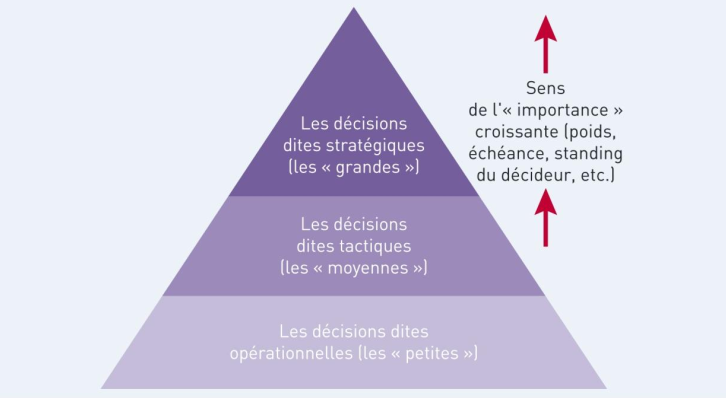
\includegraphics[width=\textwidth]{niveaudeladecision}
    \caption{Les niveaux de la décision}
    \label{fig:niveaudeladecision}
\end{figure}


Pour les décisions moins importantes, les chefs des différents départements ou services peuvent s’en charger suivant le même procédé que celui mentionné plus haut. En gros on recueille les points suivants dans la procédure de prise de décision.
\begin{itemize}
    \item Identifier la problématique à résoudre
    \item Identifier les différentes options possibles (brainstormings)
    \item Analyser les conséquences pour chaque option (analyses des chiffres)
    \item Définir l'option retenue (le directeur) et la mettre en oeuvre (les acteurs concernés)
\end{itemize}

\subsection{Critique de l’existant}
La critique de l'existant, appelée aussi bilan de l'existant, va nous aider à l'évaluation du système existant par rapport à la prise de décisions de gestion commerciale puisque c'est là que se pose nos problématiques. Ce diagnostic est établit dans le but de rechercher des solutions futures à des problèmes posés.
\paragraph{}
Le but de la critique de l'existant est d'établir un diagnostic précis sur les procédures utilisées, relever les anomalies, les qualités et les défauts du système existant.
\paragraph{}
Par ailleurs, deux aspects sont toujours dégagés lors de cette critique dont l'un est positif et l'autre négatif.Ces deux aspects méritent d'être soulevés étant donné que le besoin de la perfection sera toujours souhaité par les utilisateurs en vue de bon fonctionnement.

\subsubsection{Aspect(s) positifs}
Sous forme de liste on peut recenser les points positifs suivants dans le processus de prise de décisions.
\begin{itemize}
    \item Les opinions et analyses sont collectives
    \item Les chiffres (données) sont prises en considération dans le processus
    \item L'aspect \textit{"intuition"} est aussi considéré, ce qui garde notre nature humaine dans le processus.
\end{itemize}

\subsubsection{Aspect(s) négatifs}
Dans le processus de prise de décisions, l'analyse des chiffres intervient mais comme nous le savons tous, l'erreur est humaine. En ce faisant on peut rencontrer l'un des problèmes suivants, ce qui risque de mener à une mauvaise décision :

\begin{itemize}
    \item Mauvaise compréhension des chiffres
    \item Mauvaise correlation entre les différents sources ou rapports
    \item Ne pas analyser au delà des chiffres
    \item Focus sur la mauvaise métrique
\end{itemize}


\subsection{Les solutions concurrentes}
Nous avons vu plus haut les étapes du processus de prise de décisions. Il peut être reformulé de la façon suivante :
\begin{itemize}
    \item La phase de formulation ;
    \item La phase d’instruction ;
    \item La phase de choix ;
    \item La phase d’exécution.
\end{itemize}
\subsubsection{Techniques de prise de décisions}
Dans le processus mentionné plus haut c’est la troisième phase qui nous intéresse ici. On recense les techniques suivantes pour passer cette phase :
\begin{itemize}
    \item Se fier à l’intuition d’une ou plusieurs personnes
    \item Analyser les chiffres
    \item Utiliser un outil d’aide à la décision (Business Intelligence)
\end{itemize}

Nous avons vu plus haut quelques problèmes sur lesquels nous pouvons tomber en simplement analysant les chiffres sans outil d’aide. Aussi, l’intuition humaine peut s’avérer important dans certaines situations mais il est loin d’être suffisant pour prendre des décisions importantes. Nous pouvons ainsi conclure qu’un outil d’aide à la décision s’impose si nous voulons être optimal dans nos prises de décisions.

\subsubsection{Typologies des solutions de Business Intelligence}
\begin{itemize}
    \item \textbf{BI intégrée :} Il s’agit de solutions pouvant être intégrées à d’autres applications. Elle offrent des fonctionnalités analytiques et génèrent rapports et tableaux de bords ad hoc. Leur grande force réside dans leur capacité à s’intégrer à l’existant, y compris aux solutions de gestion d’éditeurs différents.
    \item \textbf{BI en libre service :} Il s’agit de solutions orientées utilisateur final : il n’a pas à se soucier du traitement en amont des données. Par le biais d’une interface conviviale, il peut librement explorer les données disponibles via des tableaux de bords personnalisables. On qualifie parfois ces solutions d’auto-suffisantes car elles accèdent à différentes sources de données pour en extraire des informations pertinentes sans le concours d’un service informatique dédié.
    \item \textbf{La DataViz :} Il s’agit de la data visualisation (visualisation de données) une fonction essentielle dans le traitement graphique des données traitées par la BI. Il s’agit de rendre intelligibles les informations traitées sous formes de graphes, tableaux et autres histogrammes. L’utilisateur final peut à loisir opter pour la visualisation qui correspond au traitement attendu des données. Contrairement à d’autres solutions, les applications de DataViz ne se connectent pas à des entrepôts de données non-structurées mais utilisent des bases de données déjà établies et/ou les données issues d’applications métiers. Il s’agit de fournir des indicateurs précis en temps réel afin de saisir un instantané opérationnel. La plupart du temps les tableaux de bord offrent une interface qui permet de les modifier par simple glisser-déposer.
    \item \textbf{Plate-forme de Business Intelligence : } Il s’agit d’outils complets de traitement des données structurées et non-structurées. Ils exploitent ces dernières afin d’en tirer une analyse pertinente, traduite elle aussi sous forme graphique. Ce type de solutions nécessite souvent un travail de développement et des spécialistes au sein d’un service informatique qui géreront le traitement des données en amont de l’utilisateur métier. Ce dernier peut alors se consacrer pleinement à l’analyse métier.
\end{itemize}
Nous avons plusieurs sources de données de différents types, nous voulons pouvoir faires des analyses et enfin visualiser ces données. Après cette étude nous sommes ressortis avec le tableau \ref{tab:comparatiftypebi} comparant les différents types de BI. Ceci nous guidera dans notre choix du type de solution à adopter.

\begin{table}[H]
    \centering
    \caption{Tableau comparatif des types de Business Intelligence.}
    \begin{tabular}[t]{|p{6cm}|p{3cm}|p{3cm}|p{3cm}|} 
        \hline
        \textbf{Typologie} & \textbf{Agrégation} & \textbf{Analyse} & \textbf{Visualisation} \\
        \hline\hline
        BI intégrée & Non & Non & \textbf{Oui} \\
        \hline
        BI en libre service & Non & Non & \textbf{Oui} \\
        \hline
        La DataViz & Non & \textbf{Oui} & \textbf{Oui} \\
        \hline
        Plate-forme de Business Intelligence & \textbf{Oui} & \textbf{Oui} & \textbf{Oui} \\
        \hline\hline
    \end{tabular}
    \label{tab:comparatiftypebi}
\end{table}%



\section{Solution retenue}
Nous constatons donc que la typologie qui répond pleinement a nos attentes est la plate-forme de Business Intelligence. Nous allons donc opter pour cette option et commencer la construction de notre plate-forme.

\subsection{Description de la solution}
Le terme Business Intelligence (BI), ou informatique décisionnelle, désigne les applications, les infrastructures, les outils et les pratiques offrant l’accès à l’information, et permettant d’analyser l’information pour améliorer et optimiser les décisions et les performances d’une entreprise. Le schéma dans la figure \ref{fig:aidealadecision} extrait d'une présentation de Ronan Tournier sur ResearchGate\footnote{https://www.researchgate.net/figure/Architecture-dun-systeme-decisionnel-fig2-30514732} montre la place que le système vient occuper dans l'entreprise.

\begin{figure}[H]
    \centering
    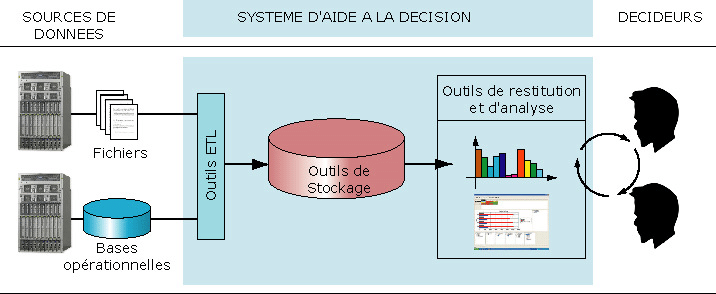
\includegraphics[width=\textwidth]{aidealadecision}
    \caption{Le système d'aide à la décision.}
    \label{fig:aidealadecision}
\end{figure}

Ainsi, la BI regroupe une large variété d’outils, d’applications et de méthodologies permettant de collecter des données en provenance de systèmes internes et de sources externes, de les préparer pour l’analyse, de les développer et de lancer des requêtes au sein de ces ensembles de données. Ces outils permettent ensuite de créer des rapports, des tableaux de bord et des visualisations de données pour rendre les résultats des analyses disponibles pour les preneurs de décisions.
\paragraph{}

De ce fait notre solution sera constitué de trois (03) grandes parties, chaqu’une pouvant être implémentée indépendamment avec des outils qui lui sont propres.  
\begin{itemize}
    \item \textbf{Agrégation des données :} Cette partie concerne la construction de l’entrepôt de donnes ou datawarehouse, à partir des multiples sources de données. On utilisera les notions d’ETL abordées plus haut dans la revue de littérature. La finalité de cette partie est un dépôt central de données structuré prêt à être utilisé à des fins d’analyse.
    \item \textbf{Analyse des données :}  Ici nous allons nous concentre sur l’aspect d’analyse des données pour en ressortir l’information souhaitée. Nous allons nous baser sur des problématiques précises pour faire nos analyses et ressortir des indicateurs. On utilisera les concepts de Datamart et cubes OLAP pour faire nos analyses. Dépendant des problématiques posées en entrée, nous en ressortons d’ici avec des indicateurs prêts à être utilise dans un outil de visualisation de données.
    \item \textbf{Reporting (Visualisation des données) :} C’est la partie la plus intéressante pour l’utilisateur final. Se basant sur des indicateurs, on conçoit des rapports et tableaux de bords personnalisables pour donner une meilleure vue a l’utilisateur sur les données. C’est ce qui permet à l’utilisateur final de mieux comprendre les données et prendre des meilleures décisions.
\end{itemize}


\subsection{Objectifs du projet final}
Après avoir posé nos problèmes et étudié comment nous allons procéder à leurs résolutions, nous pouvons à présent parler des objectifs de notre solution.

\subsubsection{Objectif général}
L’objectif général c’est de mettre sur pied une plateforme de Business Intelligence, de l’intégration des données jusqu’à la visualisation en passant par l’analyse. 

\subsubsection{Objectifs spécifiques}
La solution devra nous permettre de :
\begin{itemize}
    \item Intégrer des données provenant de diverses sources notamment, l’ERP Sage 100, Gescom v14 et des fichiers Excel.
    \item Faire des analyses multidimensionnelles sur nos données.
    \item Visualiser nos données en masse et en ad hoc.
\end{itemize}










\section{Analyse Fonctionnelle (A.F.)}
L’A.F. s’adresse aux concepteurs de produits. Il peut s’agir d’un objet matériel ou immatériel (produit industriel, objet technique, service à la personne, services financier, programme informatique dans notre cas...). Le but de l’AF est d’optimiser la conception ou la reconception de produits en s’appuyant sur les fonctions que doit réaliser le produit. Une fois les fonctions du produit identifiées et caractérisées, l’équipe de conception peut mesurer son état d’avancement et de réussite par rapport à des critères objectifs.

\subsection{La démarche d’analyse fonctionnelle (A.F.)}
L’AF n’a de sens que si elle est menée au début d’un projet. Elle permet d’éviter certains pièges classiques de la conception (aveuglement, manque d’objectivité, mauvaise gestion des priorités). Dans les faits, les premières étapes de l’AF sont générales et concernent tous les acteurs d’un même projet. C’est seulement dans un deuxième temps qu'elle devient technique, et oriente les concepteurs vers des solutions techniques. Rendant ainsi possible un dialogue entre tous les intervenants d’un projet (quels que soient leurs domaines de compétence). C’est un gage d’objectivité et de créativité dans la conduite du projet.

\subsubsection{La méthode APTE : \textbf{AP}plication aux \textbf{T}echniques d’\textbf{E}ntreprise}
La méthode APTE est une méthode « universelle » d’aide à la gestion de projets, enseignée et/ou dispensée de façon très officielle par l’APTE, cabinet conseil en management, spécialisé en Analyse de la Valeur. D'apres le site officiel de la methode\footnote{http://www.methode‐apte.com/}, elle est une interprétation française de méthodes américaines d’analyse de la valeur.

\subsubsection{Les étapes de l’A.F.}
Lors d’une démarche d’analyse fonctionnelle, les concepteurs (au sens large) du produit doivent suivre les étapes suivantes, présentées dans l’ordre chronologique.
\begin{table}[H]
    \centering
    \caption{Etapes à suivre dans l'Analyse Fonctionnelle.}
    \begin{tabular}[t]{|p{6cm}|p{9cm}|} 
        \hline
        \textbf{Outil} & \textbf{Résultat attendu}\\
        \hline\hline
        Analyse du Besoin (A.B.) & Cahier des charges du besoin (note de
        cadrage). \\
        \hline
        Analyse Fonctionnelle du Besoin (A.F.B.) & Cahier des charges fonctionnel \\
        \hline
        Analyse Fonctionnelle Technique (A.F.T.) & Cahier des charges technique (spécification
        technique).\\
        \hline\hline
    \end{tabular}
    \label{tab:etapesaf}
\end{table}%

Le tableau \ref{tab:etapesaf} ressort les étapes nécessaire à l'A.F. ainsi que le résultat dont on doit espérer à la fin de chaque étape.
\begin{itemize}
    \item L’Analyse du Besoin permet \textbf{d’exprimer le besoin}.
    \item L’Analyse Fonctionnelle du Besoin permet d’identifier les relations du produit avec son contexte d’utilisation, afin de dégager des \textbf{Fonctions de Service}, aptes à satisfaire le besoin.
    \item L’Analyse Fonctionnelle Technique permet de déterminer les \textbf{Fonctions Techniques} nécessaires aux fonctions de service. Ces fonctions techniques guident les concepteurs dans la recherche des \textbf{solutions technologiques}.
\end{itemize}
\paragraph{}
L’Analyse Fonctionnelle du Besoin porte sur les \textbf{fonctions} du produit à concevoir. Elle ne préjuge pas ni des fonctions techniques induites ni des solutions constructives capables qui seront recherchées au stade de l’Analyse Fonctionnelle Technique.
\paragraph{}
La démarche d’Analyse Fonctionnelle (AB, AFB et AFT) est collective, et doit réunir des personnes représentant tous les services et tous les métiers concernés. Cela permet à la fois plus de créativité, et d’exhaustivité dans la démarche. La réflexion doit rester la plus ouverte possible, tout au long de la démarche d’analyse.

\subsection{L'Analyse du Besoin (A.B.)}

\subsubsection{Définition}
« Un besoin est un désir (ou une nécessité) éprouvé par l’utilisateur d’un système », selon AFNOR\footnote{AFNOR - Association Française de Normalisation}
\paragraph{}
On recense deux formes principales de besoin : 
\begin{itemize}
    \item Explicite (Exprimé)
    \item Implicite (Non Exprimé)
\end{itemize}

\subsubsection{Verbalisation du besoin}
La méthode de l’Analyse du Besoin s’appuie sur deux hypothèses :
\begin{itemize}
    \item La satisfaction du besoin est réalisée par l’utilisation du produit à concevoir.
    \item Le besoin est satisfait par le changement d’état d’une matière d’œuvre.
\end{itemize}

Pour verbaliser le besoin, il faut se poser trois questions et y répondre. Le tableau ... montre, dans notre projet les questions et les réponses qui nous mèneront à la formulation de notre besoin.

\begin{table}[H]
    \centering
    \caption{Questions pour formuler le besoin.}
    \begin{tabular}[t]{|p{7cm}|p{8cm}|} 
        \hline
        \textbf{Question} & \textbf{Réponse}\\
        \hline\hline
        « \textbf{A qui} le produit rend‐il service ? » & Aux décideurs \\
        \hline
        « \textbf{Sur quoi} le produit agit‐il ? » & Les données de gestion commerciale \\
        \hline
        « \textbf{Dans quel but} ? » & Améliorer la prise de décisions\\
        \hline\hline
    \end{tabular}
    \label{tab:etapesaf}
\end{table}%

Traditionnellement dans la méthode APTE le besoin est représenté grâce à un outil graphique : le schéma du besoin (la « Bête à cornes ») illustré dans la figure \ref{fig:bac}.

\begin{figure}[H]
    \centering
    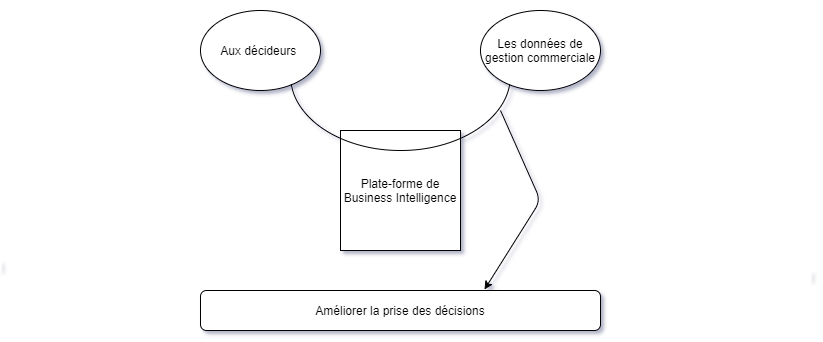
\includegraphics[width=\textwidth]{bac}
    \caption{Diagramme bête à cornes}
    \label{fig:bac}
\end{figure}

Les réponses à ces trois questions aboutissent à un énoncé du besoin, qui peut être formulé comme suit :

\textbf{« La plate-forme de Business Intelligence rend service aux décideurs de AMD Sarl en agissant sur les données de gestion commerciale pour améliorer la prise des décisions »}.



\subsection{L'Analyse Fonctionnelle du Besoin (A.F.B.)}
L'A.F.B est faite selon les deux hypothèses suivantes :
\begin{itemize}
    \item Le besoin est satisfait par l’utilisation d’un produit.
    \item Le produit est un générateur de \textbf{services} (ou « prestations client »)
\end{itemize}

\subsubsection{Les concepts de l’A.F.B}
L’Analyse Fonctionnelle du Besoin est appelée ainsi car elle va permettre de traduire le besoin en des fonctions à réaliser : les \textbf{Fonctions de Service}. L'A.F.B. est aussi appelée Analyse Fonctionnelle Externe.
\paragraph{Notion de Fonctions de Service (F.S.)}
Définition d’une fonction suivant la norme AFNOR X50‐151 :
\textbf{« Action d'un produit ou de l'un de ses constituants exprimée exclusivement en termes de finalité ».}
\subparagraph{}
On peut l'interpreter comme une action du produit avec son milieu extérieur, qui contribue à la satisfaction du besoin (identifié et caractérisé lors de l’A.B.). On ne peut identifier et caractériser les fonctions de service que si l’on a au préalable \textbf{identifié et caractérisé le milieu extérieur} du produit. Le milieu extérieur du produit à concevoir dépend de l’instant auquel on le considère. Le cycle de vie du produit étant constitué de multiples étapes, on doit identifier le \textbf{milieu extérieur correspondant à chaque phase de vie du produit.}

\paragraph{Les étapes de l’A.F.B.}
L’Analyse Fonctionnelle du Besoin est une démarche relativement longue, qui conditionne
grandement la réussite du projet et demande donc beaucoup de rigueur et de soin.
\begin{itemize}
    \item Identification des \textbf{phases de vie} du produit
    \item Pour chaque phase de vie (à minima les principales) :
    \begin{itemize}
        \item Identification et caractérisation des \textbf{Eléments du Milieu Extérieur (E.M.E.)}
        \item Identification des Fonctions de Service (F.S.)
        \item Caractérisation des F.S.
    \end{itemize}
    \item Rédaction du \textbf{cahier des charges fonctionnel}
\end{itemize}

\subsubsection{Phases de vie du produit}
Suivant les objectifs de la conception et le niveau de précision recherché, on peut identifier
de très nombreuses phases de vie pour un produit.

On peut avoir conception, fabrication, tests d’intégration, conditionnement, transport, commercialisation, montage, installation / mise en œuvre, validation, utilisation normale (principale), utilisation normale (secondaire), utilisation anormale (mode dégradé), maintenance, non utilisation, stockage, reconditionnement, mise à jour, recyclage / destruction. Cete liste est non exhaustive.

Dépendant des objectifs du  produit on peut choisir les phases de vie de notre produit.

Notre produit est une solution informatique. On peut donc se baser sur le cycle de vie d'un logiciel informatique déjà conçu pour choisir les phases de vie de notre produit.

On peut donc choisir les suivants : 
\begin{itemize}
    %\item conception
    \item utilisation
    \item mise à jour
\end{itemize}

\subsubsection{Eléments du Milieu Extérieur (E.M.E.)}
Pour identifier les fonctions du produit, il faut être capable de décrire son environnement (appelé « Milieu Extérieur »). Toutes les entités qui sont identifiées comme extérieures au produit
sont appelées \textbf{Eléments du Milieu Extérieur : E.M.E.}. Les E.M.E. doivent être identifiés pour chaque phase de vie étudiée!

Pour ce faire il faut identifier les éléments intervenant dans chaque phase de vie et en déterminer les E.M.E. Un E.M.E. doit pouvoir être défini de façon objective pour tous les protagonistes de l’étude. Si on ne peut pas définir entièrement un élément par des critères objectifs, alors cet élément n’est pas un élément du milieu extérieur. Le choix d’un E.M.E. conditionnera l’énoncé des Fonctions de Service.

% \paragraph{Phase de conception}
% Ici on peut identifier comme éléments dans l'environnement du produit les suivants:
% \begin{itemize}
%     \item Outils de conception
%     \item Modèle de données
%     \item Concepteur
%     \item Normes de sécurité 
%     \item Règles de qualité
% \end{itemize}
% On aura donc un diagramme comme dans la figure \ref{fig:emeconception}


% \begin{figure}[H]
%     \centering
%     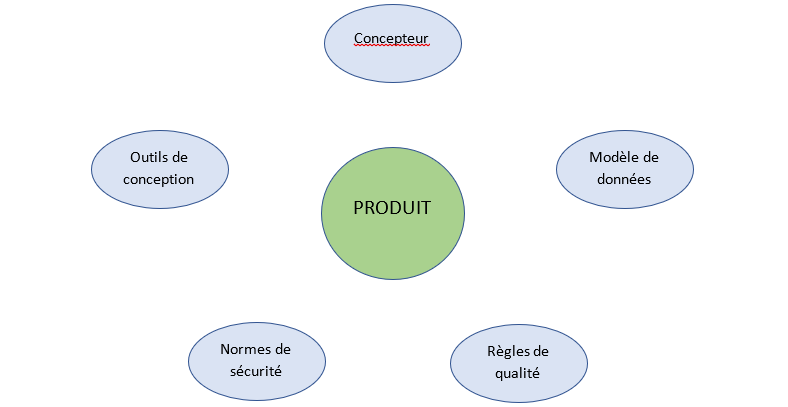
\includegraphics[width=\textwidth]{emeconception}
%     \caption{Identification des E.M.E. dans la phase Conception}
%     \label{fig:emeconception}
% \end{figure}

\paragraph{Phase d'utilisation}
Ici on peut identifier comme éléments dans l'environnement du produit les suivants:
\begin{itemize}
    \item Client 
    \item Données
    \item Décisions
    \item Normes de sécurité 
    \item Normes d'ergonomie
    \item Règles de qualité
\end{itemize}
On aura donc un diagramme comme dans la figure \ref{fig:emeutilisation} représentant les E.M.E.

\begin{figure}[H]
    \centering
    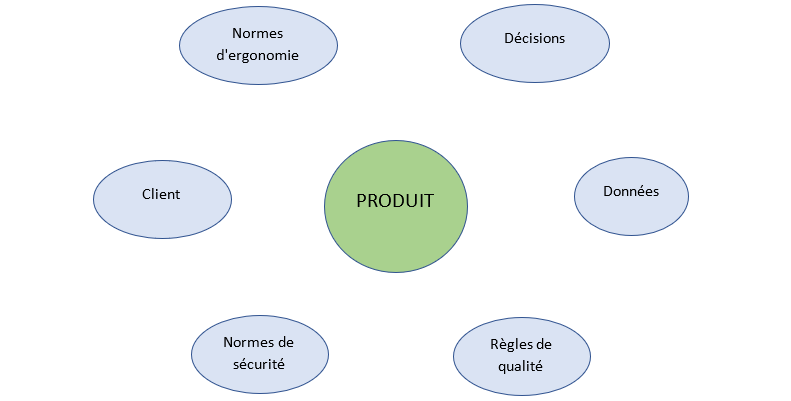
\includegraphics[width=\textwidth]{emeutilisation}
    \caption{Identification des E.M.E. dans la phase Développement}
    \label{fig:emeutilisation}
\end{figure}



\paragraph{Phase de mise à jour}
Ici on peut identifier comme éléments dans l'environnement du produit les suivants:
\begin{itemize}
    \item Client (Décideurs) 
    \item Données 
    \item Décisions 
    \item Concepteur
    \item Normes de sécurité 
    \item Normes d'ergonomie
    \item Règles de qualité
\end{itemize}
Ici on peut constater que le client et les données en sont pas intrinsèquement liées à la phase de mise à jour. On a donc Client et Données comme E.M.E. ici. On aura donc un diagramme comme dans la figure \ref{fig:ememiseajour}.


\begin{figure}[H]
    \centering
    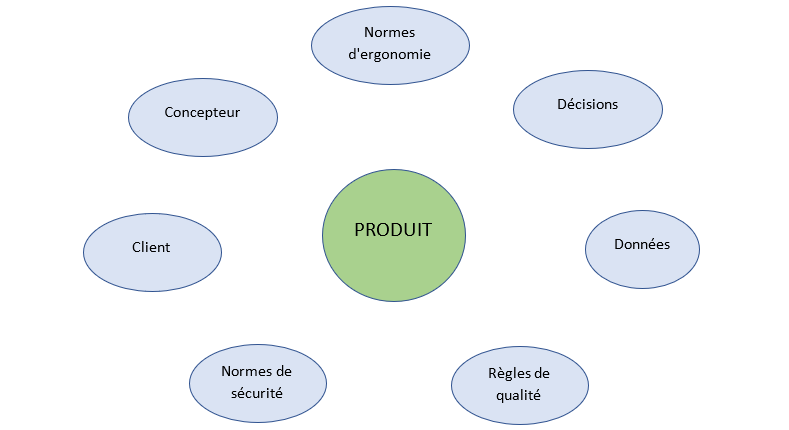
\includegraphics[width=\textwidth]{ememiseajour}
    \caption{Identification des E.M.E. dans la phase Mise A Jour}
    \label{fig:ememiseajour}
\end{figure}



\subsubsection{Fonctions de Service (F.S.)}
On identifie les Fonctions de Service grâce à un outil graphique : le graphe des interacteurs,
ou graphe fonctionnel (le « Diagramme Pieuvre » de la méthode APTE) :
\begin{itemize}
    \item Les relations du produit avec son milieu extérieur (pour une phase de vie donnée) sont représentées par des traits.
    \item Chaque trait correspond à une Fonction de Service (F.S.)
    \item Chaque trait doit relier le produit à un EME ou bien relier plusieurs EME en passant par le produit.
\end{itemize}

\paragraph{Classification des Fonctions de Service}
\begin{itemize}
    \item \textbf{Fonctions Principales (F.P) : \textit{« Fonction de service qui met en relation deux EME (ou plus), via le produit »}.} Les fonctions principales traduisent obligatoirement des actions réalisées par le produit. Il peut être nécessaire de mettre en relation plus de deux EME par une seule fonction principale, mais c’est un cas à éviter dans la mesure du possible.
    \item \textbf{Fonctions Contraintes (F.C) : \textit{« Fonction de service qui met en relation le produit avec un seul EME »}.} Chaque EME doit être relié au produit par au moins une fonction contrainte. Les fonctions contraintes traduisent la plupart du temps une adaptation du produit à son milieu
    extérieur.
\end{itemize}

\paragraph{L’expression des fonctions est normalisée par l’AFNOR :} Une fonction se compose d'un \textbf{verbe} ou d'un \textbf{groupe verbal caractérisant l'action}, et de compléments représentant les \textbf{éléments du milieu extérieur} concernés par la fonction. Le sujet de la phrase n'apparait pas, mais il renvoie toujours au produit.

Outre cette définition formelle, certaines règles d'usage sont à respecter :
\begin{itemize}
    \item les formes passive et négative sont à éviter (forme passive admise pour les contraintes)
    \item la formulation de la fonction doit être indépendante des solutions susceptibles de la réaliser
    \item la formulation doit être la plus concise et la plus claire possible
\end{itemize}


\paragraph{Fonctions de service pour la phase d'utilisation}

\begin{figure}[H]
    \centering
    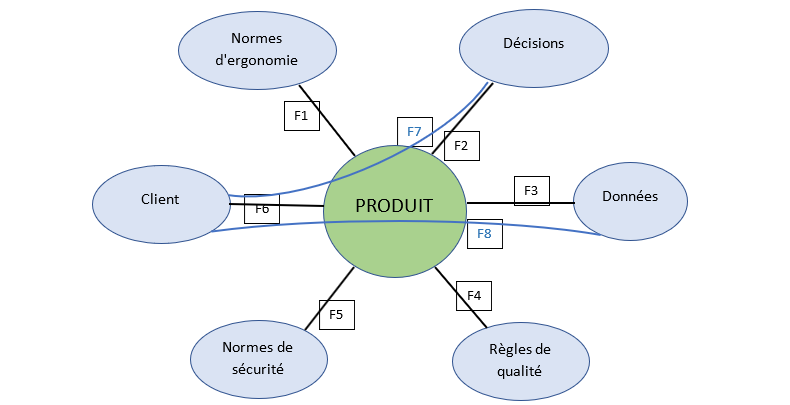
\includegraphics[width=\textwidth]{fsutilisation}
    \caption{Diagramme Pieuvre (Identification des F.S) dans la phase Utilisation}
    \label{fig:fsutilisation}
\end{figure}

On peut formuler 8 fonctions de services d’après le diagramme de la figure \ref{fig:fsutilisation}
\begin{itemize}
    \item Respecter les normes d’ergonomie
    \item Permettre une meilleure prise de décisions
    \item Analyser les données
    \item Respecter les règles de qualité 
    \item Respecter les normes de sécurité
    \item Fournir des indicateurs au client
    \item Permettre au client de prendre les décisions
    \item Permettre au client d'agréger les données
\end{itemize}



\paragraph{Fonctions de service pour la phase de Mise A Jour}

\begin{figure}[H]
    \centering
    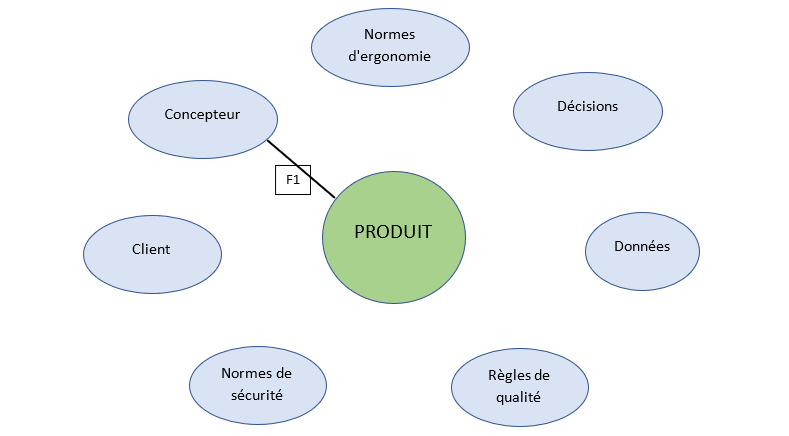
\includegraphics[width=\textwidth]{fsmiseajour}
    \caption{Diagramme Pieuvre (Identification des F.S) dans la phase Mise A Jour}
    \label{fig:fsmiseajour}
\end{figure}



Ici on complémente juste le diagramme precedent. On peut identifier la F.S. suivante dans la figure \ref{fig:fsmiseajour}.
\begin{itemize}
    \item Permettre sa mise à jour par le concepteur
\end{itemize} 



\subsubsection{Le Cahier des Charges Fonctionnel (CdCF)}
Le Cahier des Charges Fonctionnel (CdCF) est le document qui récapitule la démarche et les résultats de l’Analyse Fonctionnelle du Besoin. Il porte donc essentiellement sur les Fonctions de Service. Le CdCF fait office de contrat à respecter par les concepteurs. On doit retrouver dans le CdCF toutes les étapes de la démarche décrite dans ce chapitre :
\begin{itemize}
    \item Identification des phases de vie du produit
    \item Pour chaque phase de vie :
    \begin{itemize}
        \item Identification des EME
        \item Identification des FS 
    \end{itemize}
\end{itemize}

\paragraph{Cahier des Charges Fonctionnel}
\subparagraph{Phases de vie du produit}
\begin{itemize}
    \item Phase d'utilisation
    \item Phase de mise à jour
\end{itemize}
\subparagraph{Eléments du Milieu Extérieur (Cumulé)}
\begin{itemize}
    \item Client (Décideurs) 
    \item Données 
    \item Décisions 
    \item Concepteur
    \item Normes de sécurité 
    \item Normes d'ergonomie
    \item Règles de qualité
\end{itemize}
\subparagraph{Fonctions de Service (Cumulé)}
\begin{itemize}
    \item FS1 - Respecter les normes d’ergonomie
    \item FS2 - Permettre une meilleure prise de décisions
    \item FS3 - Analyser les données
    \item FS4 - Respecter les règles de qualité 
    \item FS5 - Respecter les normes de sécurité
    \item FS6 - Fournir des indicateurs au client
    \item FS7 - Permettre au client de prendre les décisions
    \item FS8 - Permettre au client d'agréger les données
    \item FS9 - Permettre sa mise à jour par le concepteur
\end{itemize}



\subsection{L'Analyse Fonctionnelle Technique (A.F.T.)}

\subsubsection{Définition et intérêt}
L’Analyse Fonctionnelle Technique (A.F.T.) permet de faire la transition entre l’Analyse Fonctionnelle du Besoin (qui reste étrangère aux préoccupations d’ordre technologiques) et la conception détaillée, qui entre de plain pied dans les considérations technologiques. L’Analyse Fonctionnelle Technique est aussi appelée \textbf{Analyse Fonctionnelle interne.}

\paragraph{Intérêts de l’AFT}
\begin{itemize}
    \item \textbf{L’approche systémique : } L’AFT permet une approche systémique de la recherche de solutions technologiques. 
    \item \textbf{La traçabilité : } Les outils de l’AFT permettent aux concepteurs d’associer immédiatement (grâce à son nom) toute Fonction Technique (F.T.) et toute Solution Technologique (S.T.) à la Fonction de Service (F.S.) qui la justifie. Cela permet un suivi optimal du projet/produit durant toute sa vie, y compris pour les évolutions du produit. Si l’on connaît les Fonctions de Service qui sont modifiées, on connaît immédiatement les Solutions Technologiques qui sont impactées par ces modifications.
\end{itemize}



\subsubsection{Le diagramme FAST}
Pour mener une Analyse Fonctionnelle Technique, il existe un outil principal : le F.A.S.T.
(acronyme de « Functionnal Analysis System Technique »). D’autres outils existent, mais il s’agit de
compléments au FAST.

\paragraph{Notion de Fonction Technique :} Une Fonction Technique (F.T.) est une fonction contribuant à réaliser une fonction de service par un moyen technique. Une FT s’énonce nécessairement avec un verbe à l’infinitif. Ce verbe doit être, autant que possible, un verbe d’action.
\begin{itemize}
    \item Toutes les fonctions de service ne peuvent pas être décrites par des FT. Par exemple, une fonction contrainte du type « Respecter la norme », si elle est bien caractérisée, se suffit à elle‐même.
    \item Si l’on n’arrive pas à énoncer une FT avec un verbe d’action, il y a de grandes chances pour que l’on soit en train de faire fausse route.
\end{itemize}

\paragraph{Utilisation du FAST :} Les fonctions, représentées par des blocs rectangulaires, sont liées entre elles par des traits droits (sans flèches), qui les ordonnent. Les fonctions techniques sont nommées \textbf{FT}\textit{ijk}… où i est le numéro de la FS développée (FSi). j et k indiquent la position de la fonction technique dans
l’arborescence de FSi.

Après avoir éliminé les F.S. qui ne respectent pas les règles de formulation de F.T. on peut recenser les F.T. suivants
\begin{itemize}
    \item FS2 - Permettre une meilleure prise de décisions 
    \begin{itemize}
        \item Construire des tableaux de bord
        \item Construire des rapports détaillés
    \end{itemize}
    \item FS3 - Analyser les données
    \begin{itemize}
        \item Construire les cubes de données 
    \end{itemize}
    \item FS8 - Permettre au client d’agréger les données
    \begin{itemize}
        \item Construire un entrepôt de données
    \end{itemize}
\end{itemize}


Image du tableau FAST



\section{Gestion du projet }
\subsection{Processus de développement }
Le processus de développement ou encore cycle de vie, c'est l'ensemble structuré d'activités à réaliser pour atteindre l'objectif d'un projet SI, dont les activités varient en fonction de l'organisation, du projet, et du type de système à développer. Ce processus doit être explicitement décrit pour être adéquatement géré. 
\paragraph{}
Le \textbf{cycle de vie d'un SI} décrit succintement les phases par lesquelles passe un système d'information depuis le \textbf{besoin initial} jusqu'au \textbf{retrait du système}, la documentation et les décisions qui jalonnent le cycle.

\subsubsection{Activités de développement des SI}
\begin{itemize}
    \item \textbf{Spécification} des exigences et des contraintes du système, établissement du cahier des charges
    \item \textbf{Conception} de la solution, production d'un modèle du système à développer
    \item \textbf{Implémentation} du système
    \item \textbf{Test} du système, vérification de l'adéquation entre les propriétés implémentées du système et la spécification des besoins
    \item \textbf{Installation} du système chez le client et vérification de son fonctionnement
    \item \textbf{Maintenance} du système, réparation des fautes
\end{itemize}

\subsubsection{Importance du processus de développement des SI}
Il est important de structurer les phases impliquées dans les efforts de développement de logiciels et le processus de développement sert cet objectif. Le processus de développement ne se termine que lorsque toutes les phases ont été accomplies avec succès. Tous les besoins potentiels doivent être ajustés au sein du système. L'avantage le plus visible du processus de développement est qu'il permet de contrôler dans une certaine mesure les activités de développement et de garantir que le système logiciel est conforme à toutes les exigences estimées. 


\subsubsection{Types de processus de développement}
Il existe plusieurs modèles de cycle de vie (processus de développement) permettant de développer ou de produire des systèmes d’information. Ces modèles ont pour but de détecter les erreurs au pus tôt et ainsi de maitriser la qualité du produit et les délais de réalisation et ainsi que les coûts de réalisation. On peut regrouper ces modèles de cycle de vie en trois catégories soit :
\begin{itemize}
    \item \textbf{Les modèles linéaires :}  Il se compose d'un certain nombre de phases qui sont exécutées dans un ordre séquentiel sans boucles de rétroaction. Il ne produit une solution qu'à la fin phase.
    \item \textbf{Les modèles itératifs :} Il se compose d'un certain nombre de phases qui sont répétés en groupes avec un feedback après l'exécution de chaque groupe.
    \item \textbf{Les modèles agiles :} Modèle adaptatif, progresse d'itération en itération basé sur une spécification limitée de la solution. Chaque itération apprend des précédentes et redirige l'tération suivante pour tenter de converger vers la meilleure solution possible capabl de satisfaire le client.
\end{itemize}

Aujourd’hui, la catégorie des méthodes agile est plus répandue par rapport aux deux autres car elle permet l’aboutissement d’un produit qui satisfait mieux le client, plus facilement modifiable et beaucoup moins couteux pour la maintenance et la mise a jour que les autres.\\
Dans cette catégorie nous pouvons recenser quelques-uns des méthodes les plus utilisées :


\begin{itemize}
    \item \textbf{Méthodologie Agile Scrum : } Scrum  est un cadre de gestion de projet Agile léger qui peut être utilisé pour gérer des projets itératifs et incrémentiels de tous types. Il a gagné en popularité au fil des ans en raison de sa simplicité, de sa productivité éprouvée et de sa capacité à intégrer diverses pratiques globales promues par d'autres modèles Agile.
    \item \textbf{Kanban : } Kanban  est une méthode de gestion de flux de travail hautement visuelle qui est populaire parmi les équipes Lean. En effet, 83\% des équipes pratiquant le Lean utilisent Kanban pour visualiser et gérer activement la création de produits en mettant l'accent sur la livraison continue, sans ajouter plus de stress au cycle de vie du développement logiciel.
    \item \textbf{Extreme Programming (XP) : } XP est une approche disciplinée pour le développement de logiciels agiles de haute qualité, axée sur la rapidité et la livraison continue. Il vise à améliorer la qualité et la réactivité des logiciels face à l'évolution des exigences des clients. Il favorise une forte implication des clients, de feedback rapide, des tests continus, une planification continue et un travail d'équipe étroit pour fournir des logiciels fonctionnels à des intervalles très fréquents, généralement toutes les 1 à 3 semaines.
\end{itemize}

Pour ce projet nous utiliseront la méthodologie SCRUM car elle est la plus adaptée pour la gestion de notre projet.

% \subsection{Choix des outils de modélisation}
% \blindtext


\subsection{Outils et techniques de gestion}
\subsubsection{Présentation du processus de développement agile : SCRUM}
\paragraph{Principes de SCRUM}
Scrum est considéré comme un cadre ou « framework » de gestion de projet. Ce cadre est constitué d'une définition des rôles, de réunions et d'artefacts.

Scrum définit 3 rôles :​
\begin{itemize}
    \item \textbf{Le « Product Owner »} qui porte la vision du produit à réaliser (représentant généralement le client).
    \item \textbf{Le « Scrum Master »} garant de l'application de la méthodologie Scrum.
    \item \textbf{L'équipe de développement} qui réalise le produit.
\end{itemize}

\paragraph{Cycle de vie SCRUM}
\subparagraph{Un peu de vocabulaire :}
\begin{itemize}
    \item \textbf{Product backlog (Backlog produit) : } Une liste priorisée de besoins et exigences que veut le client, exprimé dans son vocabulaire et sa terminologie métier, souvent en termes de scénarios (user stories).
    \item \textbf{User story (scénario) : }Le scénario est une exigence du système à développer, formulée en une ou deux phrases dans le langage de l'utilisateur. Ces user stories émergent au cours d'ateliers de travail menés avec le Métier, le Client et/ou les utilisateurs.
    \item \textbf{Sprint backlog : }Une liste de tâches identifiées par l'équipe du projet à réaliser pendant un sprint afin d'implémenter les scénarios sélectionnés pour ce sprint.
    \item \textbf{Daily scrum : }Chaque jour on organise une courte réunion (15 minutes) pour fixer et/ou ajuster les objectifs de la journée.
\end{itemize}

La vie d'un projet Scrum est rythmée par un ensemble de réunions clairement définies et strictement limitées dans le temps (timeboxing):
\begin{itemize}
    \item \textbf{Planification du Sprint (Sprint = itération) :} Au cours de cette réunion, l'équipe de développement sélectionne les éléments prioritaires du \textbf{« Product Backlog »} (liste ordonnancée des exigences fonctionnelles et non fonctionnelles du projet) qu'elle pense pouvoir réaliser au cours du sprint (en accord avec le \textbf{« Product Owner »}).
    \item \textbf{Revue de Sprint : } Au cours de cette réunion qui a lieu à la fin du sprint, \textbf{l'équipe de développement} présente les fonctionnalités terminées au cours du sprint et recueille les feedbacks du \textbf{Product Owner} et des utilisateurs finaux. C'est également le moment d'anticiper le périmètre des prochains sprints et d'ajuster au besoin la planification de release (nombre de sprints restants).
    \item \textbf{Rétrospective de Sprint : }La rétrospective qui a généralement lieu après la revue de sprint est l'occasion de s'améliorer (productivité, qualité, efficacité, conditions de travail, etc) à la lueur du "vécu" sur le sprint écoulé (principe d'\textbf{amélioration continue}).
    \item \textbf{Mêlée quotidienne : }il s'agit d'une réunion de synchronisation de l'équipe de développement qui se fait debout (elle est aussi appelée "stand up meeting") en 15 minutes maximum au cours de laquelle chacun répond principalement à 3 questions : « Qu'est ce que j'ai terminé depuis la dernière mêlée ? Qu'est ce que j'aurai terminé d'ici la prochaine mêlée ? Quels obstacles me retardent ? »
\end{itemize}
\begin{figure}[H]
    \centering
    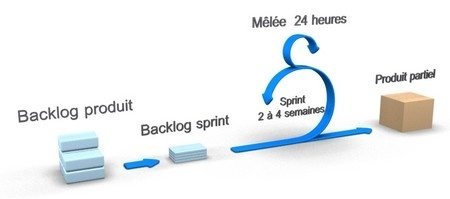
\includegraphics[width=\textwidth]{scrum}
    \caption{Cycle de vie de SCRUM}
    \label{fig:scrum}
\end{figure}

Comme on le vois dans la figure \ref{fig:scrum}, durant chaque "sprint" (habituellement 2-4 semaines), l'équipe crée un livrable. L'ensemble des fonctionnalités du sprint viennent du "backlog" du projet, qui est un ensemble priorisé d'exigences importantes à achever. Pendant une session de planification de sprint, les exigences du sprint sont définies. Les exigences sont gelées pendant un sprint. Le sprint doit finir à temps. Si les exigences ne sont pas totalement mises en place, elles retournent au backlog du projet. Après avoir complété un sprint, l'équipe doit démontrer le fonctionnement du logiciel.

\subparagraph{Avantages : }
\begin{itemize}
    \item Économie de temps et d'argent ;
    \item Mise en place rapide et facilité de correction des possible erreurs ;
    \item Visibilité de la mise en place du projet ;
    \item Feedback en continu du client ;
    \item Facilité de copie avec les changements ;
    \item Les réunions journalières amènent à meilleure appréciation de la productivité individuelle ;
    \item Les problèmes sont identifiés dans les premières étapes, de manière à être résolus plus rapidement ;
    \item Il est plus facile de livrer un produit de qualité durant un temps planifié.
\end{itemize}

\subsubsection{Technique d’estimation des coûts}
Afin d’évaluer le coût de notre projet, on doit d’abord définir les éléments de base qui constitue votre projet : 
\begin{itemize}
    \item Le planning initial du projet
    \item La durée de chaque tâche
    \item La durée totale du projet
    \item Les ressources humaines nécessaire
    \item Les ressources matérielles nécessaire
    \item Les ressources logiciels nécessaire
\end{itemize}

\paragraph{Méthodes d’estimation des coûts : }On distingue deux méthodes
\begin{itemize}
    \item \textbf{La méthode analogique :} Cette méthode consiste à se référer aux coûts réels des projets similaires au vôtre et à les adapter en faisant quelques ajustements. Il est également possible de s’appuyer sur l’avis d’un chef de projet expérimenté qui a travaillé sur un projet semblable. Elle se déroule en trois étapes :
    \begin{itemize}
        \item Analyse du projet ;
        \item Recherche d’un projet similaire ;
        \item Comparaison et chiffrage.
    \end{itemize}
    \item \textbf{La méthode ascendante :} Le but de cette méthode est d’estimer le coût de chaque groupement de tâches, puis d’additionner chacune de ces estimations afin d’obtenir le coût global du projet. Cette méthode est plus précise que la précédente car elle s’appuie sur l’expérience et l’avis des personnes qui exécutent les tâches en question. Cette méthode s’utilise lors de l’élaboration du budget. Une fois que tous les éléments du projet ont été chiffrés, on les additionne afin d’obtenir le coût total du projet.
\end{itemize}

Nous optons pour la deuxième méthode pour plus de précision.

\subsubsection{Outils collaboratifs}
Des centaines d’outils collaboratifs existent pour toute sorte de collaboration. Nous allons nous attarder sur trois catégories nous permettant de mener à bien notre projet. 

\paragraph{Outil de gestion de projet : }Ici nous avons opte pour \textbf{Trello}. Cet espace collaboratif prend la forme de « boards » pour les projets ou clients et de « cards » pour les tâches. Trello vous permet ainsi de suivre l’avancée des différentes missions des prestataires. Vous pouvez, par exemple, avoir une colonne « À faire », « En cours », « Rendu » et « Validé ». Lorsque vous serez en train de travailler sur une tâche, il pourra la glisser dans « En cours », puis dans « Rendu » lorsque c’est terminé. De cette façon on peut tracer et savoir exactement l’état d’avancement du projet ainsi que des taches qui bloquant l’avancement ou même des idées susceptibles d’améliorer le projet.

\paragraph{Outil professionnel pour la communication dans l’équipe : } Nous avons choisi \textbf{Slack} ici. Slack est une application de messagerie instantanée permettant le travail collaboratif. Les conversations avec vos collaborateurs et prestataires sont organisées sous forme de chaînes et lorsque l’écrit ne suffit plus vous pouvez facilement organiser des appels audios et/ou vidéos.
 \paragraph{Outil professionnel pour les réunions : } \textbf{Skype} est un logiciel de messagerie instantanée utile pour dialoguer avec vos collaborateurs en temps réel. Vous pourrez facilement organiser des réunions, et même partager vos écrans et annoter des présentations PowerPoint. Les fonctionnalités de Skype sont très avancées pour le travail collaboratif.
\subsection{Planning prévisionnel}
\subsubsection{Planification du projet}
\blindtext

\subsection{Estimation des coûts}
\blindtext

\subsubsection{Couts de développement}
\blindtext

\subsubsection{Cout de mise en production}
\blindtext



\section*{Conclusion}%
\addcontentsline{toc}{section}{\numberline{}Conclusion}%
\blindtext


\newpage
\chapter{Analyse du Projet}

\section*{Introduction}%
\addcontentsline{toc}{section}{\numberline{}Introduction}%
Dans ce chapitre nous effectuerons l’analyse de notre projet. Nous allons commencer par présenter la méthode que nous utiliserons pour le déroulement du projet. Ensuite nous aborderons l’aspect analyse fonctionnelle du système à mettre sur pied d’où on ressortira avec une solution qu’on doit présenter.
\section{Gestion du projet }
\subsection{Processus de développement }
Le processus de développement ou encore cycle de vie, c'est l'ensemble structuré d'activités à réaliser pour atteindre l'objectif d'un projet SI, dont les activités varient en fonction de l'organisation, du projet, et du type de système à développer. Ce processus doit être explicitement décrit pour être adéquatement géré. 
\paragraph{}
Le \textbf{cycle de vie d'un SI} décrit succintement les phases par lesquelles passe un système d'information depuis le \textbf{besoin initial} jusqu'au \textbf{retrait du système}, la documentation et les décisions qui jalonnent le cycle.

\subsubsection{Activités de développement des SI}
\begin{itemize}
    \item \textbf{Spécification} des exigences et des contraintes du système, établissement du cahier des charges
    \item \textbf{Conception} de la solution, production d'un modèle du système à développer
    \item \textbf{Implémentation} du système
    \item \textbf{Test} du système, vérification de l'adéquation entre les propriétés implémentées du système et la spécification des besoins
    \item \textbf{Installation} du système chez le client et vérification de son fonctionnement
    \item \textbf{Maintenance} du système, réparation des fautes
\end{itemize}

\subsubsection{Importance du processus de développement des SI}
Il est important de structurer les phases impliquées dans les efforts de développement de logiciels et le processus de développement sert cet objectif. Le processus de développement ne se termine que lorsque toutes les phases ont été accomplies avec succès. Tous les besoins potentiels doivent être ajustés au sein du système. L'avantage le plus visible du processus de développement est qu'il permet de contrôler dans une certaine mesure les activités de développement et de garantir que le système logiciel est conforme à toutes les exigences estimées. 


\subsubsection{Types de processus de développement}
Il existe plusieurs modèles de cycle de vie (processus de développement) permettant de développer ou de produire des systèmes d’information. Ces modèles ont pour but de détecter les erreurs au pus tôt et ainsi de maitriser la qualité du produit et les délais de réalisation et ainsi que les coûts de réalisation. On peut regrouper ces modèles de cycle de vie en trois catégories soit :
\begin{itemize}
    \item \textbf{Les modèles linéaires :}  Il se compose d'un certain nombre de phases qui sont exécutées dans un ordre séquentiel sans boucles de rétroaction. Il ne produit une solution qu'à la fin phase.
    \item \textbf{Les modèles itératifs :} Il se compose d'un certain nombre de phases qui sont répétés en groupes avec un feedback après l'exécution de chaque groupe.
    \item \textbf{Les modèles agiles :} Modèle adaptatif, progresse d'itération en itération basé sur une spécification limitée de la solution. Chaque itération apprend des précédentes et redirige l'tération suivante pour tenter de converger vers la meilleure solution possible capabl de satisfaire le client.
\end{itemize}

Aujourd’hui, la catégorie des méthodes agile est plus répandue par rapport aux deux autres car elle permet l’aboutissement d’un produit qui satisfait mieux le client, plus facilement modifiable et beaucoup moins couteux pour la maintenance et la mise a jour que les autres.\\
Dans cette catégorie nous pouvons recenser quelques-uns des méthodes les plus utilisées :


\begin{itemize}
    \item \textbf{Méthodologie Agile Scrum : } Scrum  est un cadre de gestion de projet Agile léger qui peut être utilisé pour gérer des projets itératifs et incrémentiels de tous types. Il a gagné en popularité au fil des ans en raison de sa simplicité, de sa productivité éprouvée et de sa capacité à intégrer diverses pratiques globales promues par d'autres modèles Agile.
    \item \textbf{Kanban : } Kanban  est une méthode de gestion de flux de travail hautement visuelle qui est populaire parmi les équipes Lean. En effet, 83\% des équipes pratiquant le Lean utilisent Kanban pour visualiser et gérer activement la création de produits en mettant l'accent sur la livraison continue, sans ajouter plus de stress au cycle de vie du développement logiciel.
    \item \textbf{Extreme Programming (XP) : } XP est une approche disciplinée pour le développement de logiciels agiles de haute qualité, axée sur la rapidité et la livraison continue. Il vise à améliorer la qualité et la réactivité des logiciels face à l'évolution des exigences des clients. Il favorise une forte implication des clients, de feedback rapide, des tests continus, une planification continue et un travail d'équipe étroit pour fournir des logiciels fonctionnels à des intervalles très fréquents, généralement toutes les 1 à 3 semaines.
\end{itemize}

Pour ce projet nous utiliseront la méthodologie SCRUM car elle est la plus adaptée pour la gestion de notre projet.

% \subsection{Choix des outils de modélisation}
% \blindtext
\subsection{Outils et techniques de gestion}
\subsubsection{Présentation du processus de développement agile : SCRUM}
\paragraph{Principes de SCRUM}
Scrum est considéré comme un cadre ou « framework » de gestion de projet. Ce cadre est constitué d'une définition des rôles, de réunions et d'artefacts.

Scrum définit 3 rôles :​
\begin{itemize}
    \item \textbf{Le « Product Owner »} qui porte la vision du produit à réaliser (représentant généralement le client).
    \item \textbf{Le « Scrum Master »} garant de l'application de la méthodologie Scrum.
    \item \textbf{L'équipe de développement} qui réalise le produit.
\end{itemize}

\paragraph{Cycle de vie SCRUM}
\subparagraph{Un peu de vocabulaire :}
\begin{itemize}
    \item \textbf{Product backlog (Backlog produit) : } Une liste priorisée de besoins et exigences que veut le client, exprimé dans son vocabulaire et sa terminologie métier, souvent en termes de scénarios (user stories).
    \item \textbf{User story (scénario) : }Le scénario est une exigence du système à développer, formulée en une ou deux phrases dans le langage de l'utilisateur. Ces user stories émergent au cours d'ateliers de travail menés avec le Métier, le Client et/ou les utilisateurs.
    \item \textbf{Sprint backlog : }Une liste de tâches identifiées par l'équipe du projet à réaliser pendant un sprint afin d'implémenter les scénarios sélectionnés pour ce sprint.
    \item \textbf{Daily scrum : }Chaque jour on organise une courte réunion (15 minutes) pour fixer et/ou ajuster les objectifs de la journée.
\end{itemize}

La vie d'un projet Scrum est rythmée par un ensemble de réunions clairement définies et strictement limitées dans le temps (timeboxing):
\begin{itemize}
    \item \textbf{Planification du Sprint (Sprint = itération) :} Au cours de cette réunion, l'équipe de développement sélectionne les éléments prioritaires du \textbf{« Product Backlog »} (liste ordonnancée des exigences fonctionnelles et non fonctionnelles du projet) qu'elle pense pouvoir réaliser au cours du sprint (en accord avec le \textbf{« Product Owner »}).
    \item \textbf{Revue de Sprint : } Au cours de cette réunion qui a lieu à la fin du sprint, \textbf{l'équipe de développement} présente les fonctionnalités terminées au cours du sprint et recueille les feedbacks du \textbf{Product Owner} et des utilisateurs finaux. C'est également le moment d'anticiper le périmètre des prochains sprints et d'ajuster au besoin la planification de release (nombre de sprints restants).
    \item \textbf{Rétrospective de Sprint : }La rétrospective qui a généralement lieu après la revue de sprint est l'occasion de s'améliorer (productivité, qualité, efficacité, conditions de travail, etc) à la lueur du "vécu" sur le sprint écoulé (principe d'\textbf{amélioration continue}).
    \item \textbf{Mêlée quotidienne : }il s'agit d'une réunion de synchronisation de l'équipe de développement qui se fait debout (elle est aussi appelée "stand up meeting") en 15 minutes maximum au cours de laquelle chacun répond principalement à 3 questions : « Qu'est ce que j'ai terminé depuis la dernière mêlée ? Qu'est ce que j'aurai terminé d'ici la prochaine mêlée ? Quels obstacles me retardent ? »
\end{itemize}
\begin{figure}[H]
    \centering
    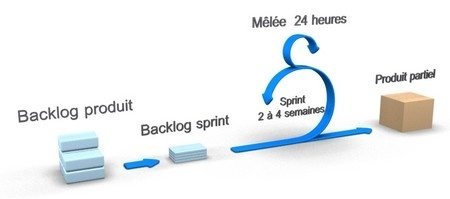
\includegraphics[width=\textwidth]{scrum}
    \caption{Cycle de vie de SCRUM}
    \label{fig:scrum}
\end{figure}

Comme on le vois dans la figure \ref{fig:scrum}, durant chaque "sprint" (habituellement 2-4 semaines), l'équipe crée un livrable. L'ensemble des fonctionnalités du sprint viennent du "backlog" du projet, qui est un ensemble priorisé d'exigences importantes à achever. Pendant une session de planification de sprint, les exigences du sprint sont définies. Les exigences sont gelées pendant un sprint. Le sprint doit finir à temps. Si les exigences ne sont pas totalement mises en place, elles retournent au backlog du projet. Après avoir complété un sprint, l'équipe doit démontrer le fonctionnement du logiciel.

\subparagraph{Avantages : }
\begin{itemize}
    \item Économie de temps et d'argent ;
    \item Mise en place rapide et facilité de correction des possible erreurs ;
    \item Visibilité de la mise en place du projet ;
    \item Feedback en continu du client ;
    \item Facilité de copie avec les changements ;
    \item Les réunions journalières amènent à meilleure appréciation de la productivité individuelle ;
    \item Les problèmes sont identifiés dans les premières étapes, de manière à être résolus plus rapidement ;
    \item Il est plus facile de livrer un produit de qualité durant un temps planifié.
\end{itemize}

\subsubsection{Technique d’estimation des coûts}
Afin d’évaluer le coût de notre projet, on doit d’abord définir les éléments de base qui constitue votre projet : 
\begin{itemize}
    \item Le planning initial du projet
    \item La durée de chaque tâche
    \item La durée totale du projet
    \item Les ressources humaines nécessaire
    \item Les ressources matérielles nécessaire
    \item Les ressources logiciels nécessaire
\end{itemize}

\paragraph{Méthodes d’estimation des coûts : }On distingue deux méthodes
\begin{itemize}
    \item \textbf{La méthode analogique :} Cette méthode consiste à se référer aux coûts réels des projets similaires au vôtre et à les adapter en faisant quelques ajustements. Il est également possible de s’appuyer sur l’avis d’un chef de projet expérimenté qui a travaillé sur un projet semblable. Elle se déroule en trois étapes :
    \begin{itemize}
        \item Analyse du projet ;
        \item Recherche d’un projet similaire ;
        \item Comparaison et chiffrage.
    \end{itemize}
    \item \textbf{La méthode ascendante :} Le but de cette méthode est d’estimer le coût de chaque groupement de tâches, puis d’additionner chacune de ces estimations afin d’obtenir le coût global du projet. Cette méthode est plus précise que la précédente car elle s’appuie sur l’expérience et l’avis des personnes qui exécutent les tâches en question. Cette méthode s’utilise lors de l’élaboration du budget. Une fois que tous les éléments du projet ont été chiffrés, on les additionne afin d’obtenir le coût total du projet.
\end{itemize}

Nous optons pour la deuxième méthode pour plus de précision.

\subsubsection{Outils collaboratifs}
Des centaines d’outils collaboratifs existent pour toute sorte de collaboration. Nous allons nous attarder sur trois catégories nous permettant de mener à bien notre projet. 

\paragraph{Outil de gestion de projet : }Ici nous avons opte pour \textbf{Trello}. Cet espace collaboratif prend la forme de « boards » pour les projets ou clients et de « cards » pour les tâches. Trello vous permet ainsi de suivre l’avancée des différentes missions des prestataires. Vous pouvez, par exemple, avoir une colonne « À faire », « En cours », « Rendu » et « Validé ». Lorsque vous serez en train de travailler sur une tâche, il pourra la glisser dans « En cours », puis dans « Rendu » lorsque c’est terminé. De cette façon on peut tracer et savoir exactement l’état d’avancement du projet ainsi que des taches qui bloquant l’avancement ou même des idées susceptibles d’améliorer le projet.

\paragraph{Outil professionnel pour la communication dans l’équipe : } Nous avons choisi \textbf{Slack} ici. Slack est une application de messagerie instantanée permettant le travail collaboratif. Les conversations avec vos collaborateurs et prestataires sont organisées sous forme de chaînes et lorsque l’écrit ne suffit plus vous pouvez facilement organiser des appels audios et/ou vidéos.
 \paragraph{Outil professionnel pour les réunions : } \textbf{Skype} est un logiciel de messagerie instantanée utile pour dialoguer avec vos collaborateurs en temps réel. Vous pourrez facilement organiser des réunions, et même partager vos écrans et annoter des présentations PowerPoint. Les fonctionnalités de Skype sont très avancées pour le travail collaboratif.
\section{Analyse Fonctionnelle (A.F.)}
L’A.F. s’adresse aux concepteurs de produits. Il peut s’agir d’un objet matériel ou immatériel (produit industriel, objet technique, service à la personne, services financier, programme informatique dans notre cas...). Le but de l’AF est d’optimiser la conception ou la reconception de produits en s’appuyant sur les fonctions que doit réaliser le produit. Une fois les fonctions du produit identifiées et caractérisées, l’équipe de conception peut mesurer son état d’avancement et de réussite par rapport à des critères objectifs.

\subsection{La démarche d’analyse fonctionnelle (A.F.)}
L’AF n’a de sens que si elle est menée au début d’un projet. Elle permet d’éviter certains pièges classiques de la conception (aveuglement, manque d’objectivité, mauvaise gestion des priorités). Dans les faits, les premières étapes de l’AF sont générales et concernent tous les acteurs d’un même projet. C’est seulement dans un deuxième temps qu'elle devient technique, et oriente les concepteurs vers des solutions techniques. Rendant ainsi possible un dialogue entre tous les intervenants d’un projet (quels que soient leurs domaines de compétence). C’est un gage d’objectivité et de créativité dans la conduite du projet.

\subsubsection{La méthode APTE : \textbf{AP}plication aux \textbf{T}echniques d’\textbf{E}ntreprise}
La méthode APTE est une méthode « universelle » d’aide à la gestion de projets, enseignée et/ou dispensée de façon très officielle par l’APTE, cabinet conseil en management, spécialisé en Analyse de la Valeur. D'apres le site officiel de la methode\footnote{http://www.methode‐apte.com/}, elle est une interprétation française de méthodes américaines d’analyse de la valeur.

\subsubsection{Les étapes de l’A.F.}
Lors d’une démarche d’analyse fonctionnelle, les concepteurs (au sens large) du produit doivent suivre les étapes suivantes, présentées dans l’ordre chronologique.
\begin{table}[H]
    \centering
    \caption{Etapes à suivre dans l'Analyse Fonctionnelle.}
    \begin{tabular}[t]{|p{6cm}|p{9cm}|} 
        \hline
        \textbf{Outil} & \textbf{Résultat attendu}\\
        \hline\hline
        Analyse du Besoin (A.B.) & Cahier des charges du besoin (note de
        cadrage). \\
        \hline
        Analyse Fonctionnelle du Besoin (A.F.B.) & Cahier des charges fonctionnel \\
        \hline
        Analyse Fonctionnelle Technique (A.F.T.) & Cahier des charges technique (spécification
        technique).\\
        \hline\hline
    \end{tabular}
    \label{tab:etapesaf}
\end{table}%

Le tableau \ref{tab:etapesaf} ressort les étapes nécessaire à l'A.F. ainsi que le résultat dont on doit espérer à la fin de chaque étape.
\begin{itemize}
    \item L’Analyse du Besoin permet \textbf{d’exprimer le besoin}.
    \item L’Analyse Fonctionnelle du Besoin permet d’identifier les relations du produit avec son contexte d’utilisation, afin de dégager des \textbf{Fonctions de Service}, aptes à satisfaire le besoin.
    \item L’Analyse Fonctionnelle Technique permet de déterminer les \textbf{Fonctions Techniques} nécessaires aux fonctions de service. Ces fonctions techniques guident les concepteurs dans la recherche des \textbf{solutions technologiques}.
\end{itemize}
\paragraph{}
L’Analyse Fonctionnelle du Besoin porte sur les \textbf{fonctions} du produit à concevoir. Elle ne préjuge pas ni des fonctions techniques induites ni des solutions constructives capables qui seront recherchées au stade de l’Analyse Fonctionnelle Technique.
\paragraph{}
La démarche d’Analyse Fonctionnelle (AB, AFB et AFT) est collective, et doit réunir des personnes représentant tous les services et tous les métiers concernés. Cela permet à la fois plus de créativité, et d’exhaustivité dans la démarche. La réflexion doit rester la plus ouverte possible, tout au long de la démarche d’analyse.

\subsection{L'Analyse du Besoin (A.B.)}

\subsubsection{Définition}
« Un besoin est un désir (ou une nécessité) éprouvé par l’utilisateur d’un système », selon AFNOR\footnote{AFNOR - Association Française de Normalisation}
\paragraph{}
On recense deux formes principales de besoin : 
\begin{itemize}
    \item Explicite (Exprimé)
    \item Implicite (Non Exprimé)
\end{itemize}

\subsubsection{Verbalisation du besoin}
La méthode de l’Analyse du Besoin s’appuie sur deux hypothèses :
\begin{itemize}
    \item La satisfaction du besoin est réalisée par l’utilisation du produit à concevoir.
    \item Le besoin est satisfait par le changement d’état d’une matière d’œuvre.
\end{itemize}

Pour verbaliser le besoin, il faut se poser trois questions et y répondre. Le tableau ... montre, dans notre projet les questions et les réponses qui nous mèneront à la formulation de notre besoin.

\begin{table}[H]
    \centering
    \caption{Questions pour formuler le besoin.}
    \begin{tabular}[t]{|p{7cm}|p{8cm}|} 
        \hline
        \textbf{Question} & \textbf{Réponse}\\
        \hline\hline
        « \textbf{A qui} le produit rend‐il service ? » & Aux décideurs \\
        \hline
        « \textbf{Sur quoi} le produit agit‐il ? » & Les données de gestion commerciale \\
        \hline
        « \textbf{Dans quel but} ? » & Améliorer la prise de décisions\\
        \hline\hline
    \end{tabular}
    \label{tab:etapesaf}
\end{table}%

Traditionnellement dans la méthode APTE le besoin est représenté grâce à un outil graphique : le schéma du besoin (la « Bête à cornes ») illustré dans la figure \ref{fig:bac}.

\begin{figure}[H]
    \centering
    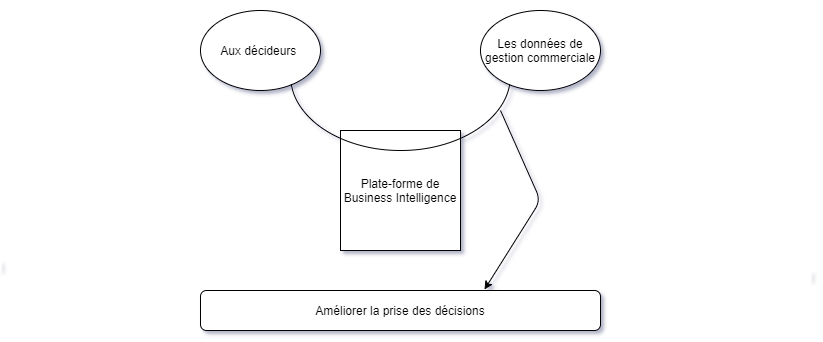
\includegraphics[width=\textwidth]{bac}
    \caption{Diagramme bête à cornes}
    \label{fig:bac}
\end{figure}

Les réponses à ces trois questions aboutissent à un énoncé du besoin, qui peut être formulé comme suit :

\textbf{« La plate-forme de Business Intelligence rend service aux décideurs de AMD Sarl en agissant sur les données de gestion commerciale pour améliorer la prise des décisions »}.



\subsection{L'Analyse Fonctionnelle du Besoin (A.F.B.)}
L'A.F.B est faite selon les deux hypothèses suivantes :
\begin{itemize}
    \item Le besoin est satisfait par l’utilisation d’un produit.
    \item Le produit est un générateur de \textbf{services} (ou « prestations client »)
\end{itemize}

\subsubsection{Les concepts de l’A.F.B}
L’Analyse Fonctionnelle du Besoin est appelée ainsi car elle va permettre de traduire le besoin en des fonctions à réaliser : les \textbf{Fonctions de Service}. L'A.F.B. est aussi appelée Analyse Fonctionnelle Externe.
\paragraph{Notion de Fonctions de Service (F.S.)}
Définition d’une fonction suivant la norme AFNOR X50‐151 :
\textbf{« Action d'un produit ou de l'un de ses constituants exprimée exclusivement en termes de finalité ».}
\subparagraph{}
On peut l'interpreter comme une action du produit avec son milieu extérieur, qui contribue à la satisfaction du besoin (identifié et caractérisé lors de l’A.B.). On ne peut identifier et caractériser les fonctions de service que si l’on a au préalable \textbf{identifié et caractérisé le milieu extérieur} du produit. Le milieu extérieur du produit à concevoir dépend de l’instant auquel on le considère. Le cycle de vie du produit étant constitué de multiples étapes, on doit identifier le \textbf{milieu extérieur correspondant à chaque phase de vie du produit.}

\paragraph{Les étapes de l’A.F.B.}
L’Analyse Fonctionnelle du Besoin est une démarche relativement longue, qui conditionne
grandement la réussite du projet et demande donc beaucoup de rigueur et de soin.
\begin{itemize}
    \item Identification des \textbf{phases de vie} du produit
    \item Pour chaque phase de vie (à minima les principales) :
    \begin{itemize}
        \item Identification et caractérisation des \textbf{Eléments du Milieu Extérieur (E.M.E.)}
        \item Identification des Fonctions de Service (F.S.)
        \item Caractérisation des F.S.
    \end{itemize}
    \item Rédaction du \textbf{cahier des charges fonctionnel}
\end{itemize}

\subsubsection{Phases de vie du produit}
Suivant les objectifs de la conception et le niveau de précision recherché, on peut identifier
de très nombreuses phases de vie pour un produit.

On peut avoir conception, fabrication, tests d’intégration, conditionnement, transport, commercialisation, montage, installation / mise en œuvre, validation, utilisation normale (principale), utilisation normale (secondaire), utilisation anormale (mode dégradé), maintenance, non utilisation, stockage, reconditionnement, mise à jour, recyclage / destruction. Cete liste est non exhaustive.

Dépendant des objectifs du  produit on peut choisir les phases de vie de notre produit.

Notre produit est une solution informatique. On peut donc se baser sur le cycle de vie d'un logiciel informatique déjà conçu pour choisir les phases de vie de notre produit.

On peut donc choisir les suivants : 
\begin{itemize}
    %\item conception
    \item utilisation
    \item mise à jour
\end{itemize}

\subsubsection{Eléments du Milieu Extérieur (E.M.E.)}
Pour identifier les fonctions du produit, il faut être capable de décrire son environnement (appelé « Milieu Extérieur »). Toutes les entités qui sont identifiées comme extérieures au produit
sont appelées \textbf{Eléments du Milieu Extérieur : E.M.E.}. Les E.M.E. doivent être identifiés pour chaque phase de vie étudiée!

Pour ce faire il faut identifier les éléments intervenant dans chaque phase de vie et en déterminer les E.M.E. Un E.M.E. doit pouvoir être défini de façon objective pour tous les protagonistes de l’étude. Si on ne peut pas définir entièrement un élément par des critères objectifs, alors cet élément n’est pas un élément du milieu extérieur. Le choix d’un E.M.E. conditionnera l’énoncé des Fonctions de Service.

% \paragraph{Phase de conception}
% Ici on peut identifier comme éléments dans l'environnement du produit les suivants:
% \begin{itemize}
%     \item Outils de conception
%     \item Modèle de données
%     \item Concepteur
%     \item Normes de sécurité 
%     \item Règles de qualité
% \end{itemize}
% On aura donc un diagramme comme dans la figure \ref{fig:emeconception}


% \begin{figure}[H]
%     \centering
%     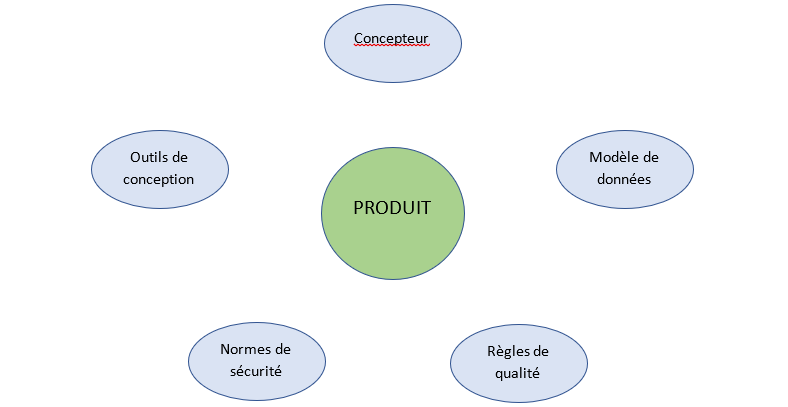
\includegraphics[width=\textwidth]{emeconception}
%     \caption{Identification des E.M.E. dans la phase Conception}
%     \label{fig:emeconception}
% \end{figure}

\paragraph{Phase d'utilisation}
Ici on peut identifier comme éléments dans l'environnement du produit les suivants:
\begin{itemize}
    \item Client 
    \item Données
    \item Décisions
    \item Normes de sécurité 
    \item Normes d'ergonomie
    \item Règles de qualité
\end{itemize}
On aura donc un diagramme comme dans la figure \ref{fig:emeutilisation} représentant les E.M.E.

\begin{figure}[H]
    \centering
    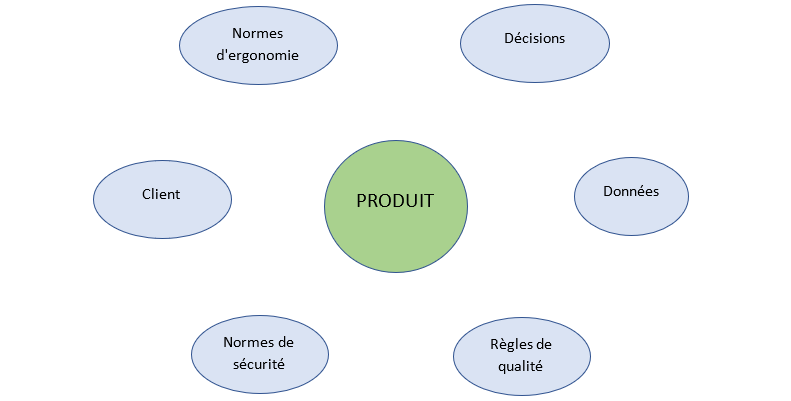
\includegraphics[width=\textwidth]{emeutilisation}
    \caption{Identification des E.M.E. dans la phase Développement}
    \label{fig:emeutilisation}
\end{figure}



\paragraph{Phase de mise à jour}
Ici on peut identifier comme éléments dans l'environnement du produit les suivants:
\begin{itemize}
    \item Client (Décideurs) 
    \item Données 
    \item Décisions 
    \item Concepteur
    \item Normes de sécurité 
    \item Normes d'ergonomie
    \item Règles de qualité
\end{itemize}
Ici on peut constater que le client et les données en sont pas intrinsèquement liées à la phase de mise à jour. On a donc Client et Données comme E.M.E. ici. On aura donc un diagramme comme dans la figure \ref{fig:ememiseajour}.


\begin{figure}[H]
    \centering
    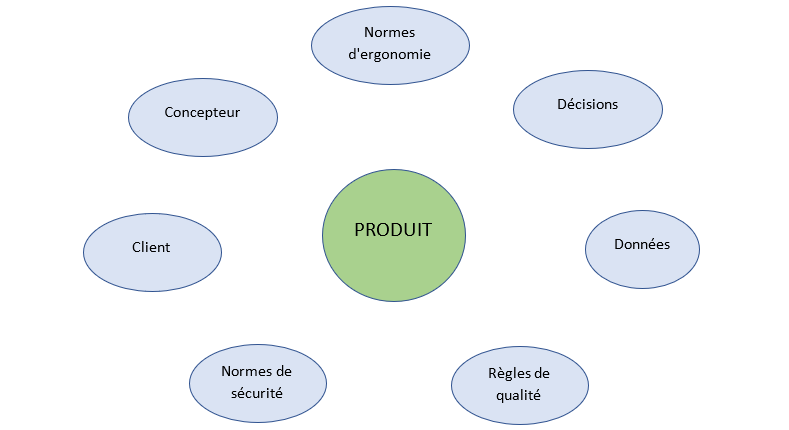
\includegraphics[width=\textwidth]{ememiseajour}
    \caption{Identification des E.M.E. dans la phase Mise A Jour}
    \label{fig:ememiseajour}
\end{figure}



\subsubsection{Fonctions de Service (F.S.)}
On identifie les Fonctions de Service grâce à un outil graphique : le graphe des interacteurs,
ou graphe fonctionnel (le « Diagramme Pieuvre » de la méthode APTE) :
\begin{itemize}
    \item Les relations du produit avec son milieu extérieur (pour une phase de vie donnée) sont représentées par des traits.
    \item Chaque trait correspond à une Fonction de Service (F.S.)
    \item Chaque trait doit relier le produit à un EME ou bien relier plusieurs EME en passant par le produit.
\end{itemize}

\paragraph{Classification des Fonctions de Service}
\begin{itemize}
    \item \textbf{Fonctions Principales (F.P) : \textit{« Fonction de service qui met en relation deux EME (ou plus), via le produit »}.} Les fonctions principales traduisent obligatoirement des actions réalisées par le produit. Il peut être nécessaire de mettre en relation plus de deux EME par une seule fonction principale, mais c’est un cas à éviter dans la mesure du possible.
    \item \textbf{Fonctions Contraintes (F.C) : \textit{« Fonction de service qui met en relation le produit avec un seul EME »}.} Chaque EME doit être relié au produit par au moins une fonction contrainte. Les fonctions contraintes traduisent la plupart du temps une adaptation du produit à son milieu
    extérieur.
\end{itemize}

\paragraph{L’expression des fonctions est normalisée par l’AFNOR :} Une fonction se compose d'un \textbf{verbe} ou d'un \textbf{groupe verbal caractérisant l'action}, et de compléments représentant les \textbf{éléments du milieu extérieur} concernés par la fonction. Le sujet de la phrase n'apparait pas, mais il renvoie toujours au produit.

Outre cette définition formelle, certaines règles d'usage sont à respecter :
\begin{itemize}
    \item les formes passive et négative sont à éviter (forme passive admise pour les contraintes)
    \item la formulation de la fonction doit être indépendante des solutions susceptibles de la réaliser
    \item la formulation doit être la plus concise et la plus claire possible
\end{itemize}


\paragraph{Fonctions de service pour la phase d'utilisation}

\begin{figure}[H]
    \centering
    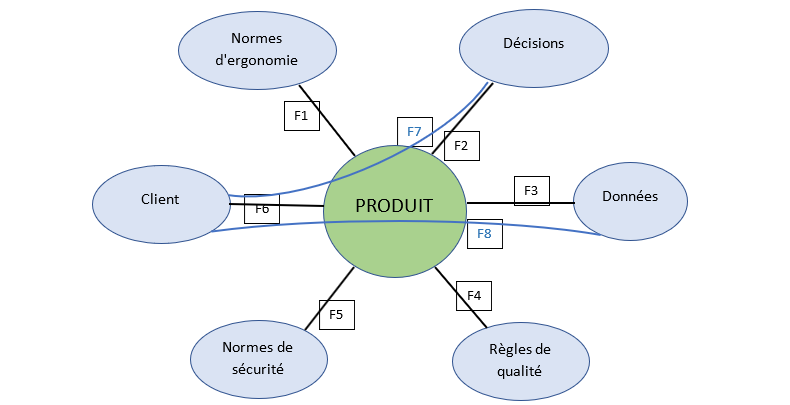
\includegraphics[width=\textwidth]{fsutilisation}
    \caption{Diagramme Pieuvre (Identification des F.S) dans la phase Utilisation}
    \label{fig:fsutilisation}
\end{figure}

On peut formuler 8 fonctions de services d’après le diagramme de la figure \ref{fig:fsutilisation}
\begin{itemize}
    \item Respecter les normes d’ergonomie
    \item Permettre une meilleure prise de décisions
    \item Analyser les données
    \item Respecter les règles de qualité 
    \item Respecter les normes de sécurité
    \item Fournir des indicateurs au client
    \item Permettre au client de prendre les décisions
    \item Permettre au client d'agréger les données
\end{itemize}



\paragraph{Fonctions de service pour la phase de Mise A Jour}

\begin{figure}[H]
    \centering
    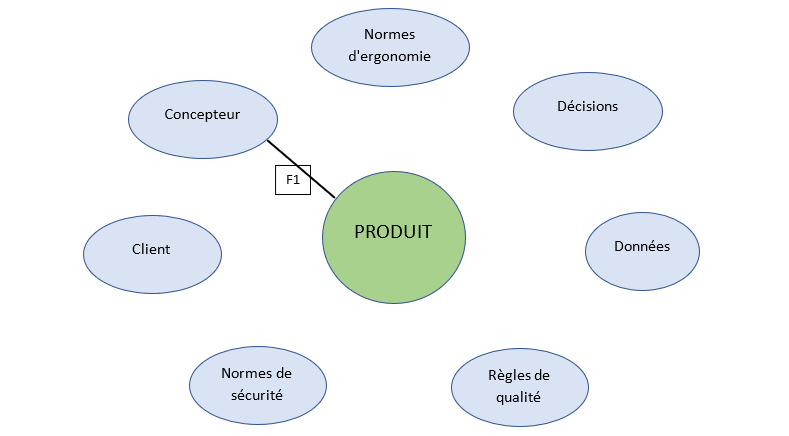
\includegraphics[width=\textwidth]{fsmiseajour}
    \caption{Diagramme Pieuvre (Identification des F.S) dans la phase Mise A Jour}
    \label{fig:fsmiseajour}
\end{figure}



Ici on complémente juste le diagramme precedent. On peut identifier la F.S. suivante dans la figure \ref{fig:fsmiseajour}.
\begin{itemize}
    \item Permettre sa mise à jour par le concepteur
\end{itemize} 



\subsubsection{Le Cahier des Charges Fonctionnel (CdCF)}
Le Cahier des Charges Fonctionnel (CdCF) est le document qui récapitule la démarche et les résultats de l’Analyse Fonctionnelle du Besoin. Il porte donc essentiellement sur les Fonctions de Service. Le CdCF fait office de contrat à respecter par les concepteurs. On doit retrouver dans le CdCF toutes les étapes de la démarche décrite dans ce chapitre :
\begin{itemize}
    \item Identification des phases de vie du produit
    \item Pour chaque phase de vie :
    \begin{itemize}
        \item Identification des EME
        \item Identification des FS 
    \end{itemize}
\end{itemize}

\paragraph{Cahier des Charges Fonctionnel}
\subparagraph{Phases de vie du produit}
\begin{itemize}
    \item Phase d'utilisation
    \item Phase de mise à jour
\end{itemize}
\subparagraph{Eléments du Milieu Extérieur (Cumulé)}
\begin{itemize}
    \item Client (Décideurs) 
    \item Données 
    \item Décisions 
    \item Concepteur
    \item Normes de sécurité 
    \item Normes d'ergonomie
    \item Règles de qualité
\end{itemize}
\subparagraph{Fonctions de Service (Cumulé)}
\begin{itemize}
    \item FS1 - Respecter les normes d’ergonomie
    \item FS2 - Permettre une meilleure prise de décisions
    \item FS3 - Analyser les données
    \item FS4 - Respecter les règles de qualité 
    \item FS5 - Respecter les normes de sécurité
    \item FS6 - Fournir des indicateurs au client
    \item FS7 - Permettre au client de prendre les décisions
    \item FS8 - Permettre au client d'agréger les données
    \item FS9 - Permettre sa mise à jour par le concepteur
\end{itemize}



\subsection{L'Analyse Fonctionnelle Technique (A.F.T.)}

\subsubsection{Définition et intérêt}
L’Analyse Fonctionnelle Technique (A.F.T.) permet de faire la transition entre l’Analyse Fonctionnelle du Besoin (qui reste étrangère aux préoccupations d’ordre technologiques) et la conception détaillée, qui entre de plain pied dans les considérations technologiques. L’Analyse Fonctionnelle Technique est aussi appelée \textbf{Analyse Fonctionnelle interne.}

\paragraph{Intérêts de l’AFT}
\begin{itemize}
    \item \textbf{L’approche systémique : } L’AFT permet une approche systémique de la recherche de solutions technologiques. 
    \item \textbf{La traçabilité : } Les outils de l’AFT permettent aux concepteurs d’associer immédiatement (grâce à son nom) toute Fonction Technique (F.T.) et toute Solution Technologique (S.T.) à la Fonction de Service (F.S.) qui la justifie. Cela permet un suivi optimal du projet/produit durant toute sa vie, y compris pour les évolutions du produit. Si l’on connaît les Fonctions de Service qui sont modifiées, on connaît immédiatement les Solutions Technologiques qui sont impactées par ces modifications.
\end{itemize}



\subsubsection{Le diagramme FAST}
Pour mener une Analyse Fonctionnelle Technique, il existe un outil principal : le F.A.S.T.
(acronyme de « Functionnal Analysis System Technique »). D’autres outils existent, mais il s’agit de
compléments au FAST.

\paragraph{Notion de Fonction Technique :} Une Fonction Technique (F.T.) est une fonction contribuant à réaliser une fonction de service par un moyen technique. Une FT s’énonce nécessairement avec un verbe à l’infinitif. Ce verbe doit être, autant que possible, un verbe d’action.
\begin{itemize}
    \item Toutes les fonctions de service ne peuvent pas être décrites par des FT. Par exemple, une fonction contrainte du type « Respecter la norme », si elle est bien caractérisée, se suffit à elle‐même.
    \item Si l’on n’arrive pas à énoncer une FT avec un verbe d’action, il y a de grandes chances pour que l’on soit en train de faire fausse route.
\end{itemize}

\paragraph{Utilisation du FAST :} Les fonctions, représentées par des blocs rectangulaires, sont liées entre elles par des traits droits (sans flèches), qui les ordonnent. Les fonctions techniques sont nommées \textbf{FT}\textit{ijk}… où i est le numéro de la FS développée (FSi). j et k indiquent la position de la fonction technique dans
l’arborescence de FSi.

Après avoir éliminé les F.S. qui ne respectent pas les règles de formulation de F.T. on peut recenser les F.T. suivants
\begin{itemize}
    \item FS2 - Permettre une meilleure prise de décisions 
    \begin{itemize}
        \item Construire des tableaux de bord
        \item Construire des rapports détaillés
    \end{itemize}
    \item FS3 - Analyser les données
    \begin{itemize}
        \item Construire les cubes de données 
    \end{itemize}
    \item FS8 - Permettre au client d’agréger les données
    \begin{itemize}
        \item Construire un entrepôt de données
    \end{itemize}
\end{itemize}


\section{Solution retenue}
Nous constatons donc que la typologie qui répond pleinement a nos attentes est la plate-forme de Business Intelligence. Nous allons donc opter pour cette option et commencer la construction de notre plate-forme.

\subsection{Description de la solution}
Le terme Business Intelligence (BI), ou informatique décisionnelle, désigne les applications, les infrastructures, les outils et les pratiques offrant l’accès à l’information, et permettant d’analyser l’information pour améliorer et optimiser les décisions et les performances d’une entreprise. Le schéma dans la figure \ref{fig:aidealadecision} extrait d'une présentation de Ronan Tournier sur ResearchGate\footnote{https://www.researchgate.net/figure/Architecture-dun-systeme-decisionnel-fig2-30514732} montre la place que le système vient occuper dans l'entreprise.

\begin{figure}[H]
    \centering
    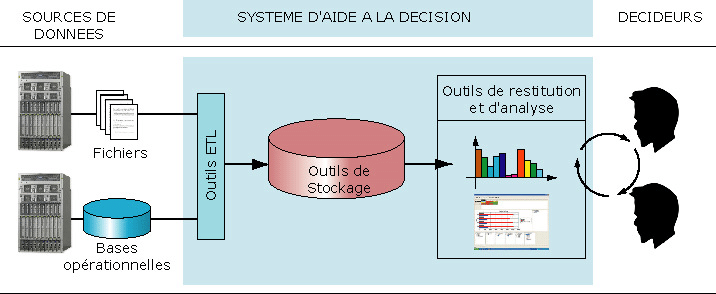
\includegraphics[width=\textwidth]{aidealadecision}
    \caption{Le système d'aide à la décision.}
    \label{fig:aidealadecision}
\end{figure}

Ainsi, la BI regroupe une large variété d’outils, d’applications et de méthodologies permettant de collecter des données en provenance de systèmes internes et de sources externes, de les préparer pour l’analyse, de les développer et de lancer des requêtes au sein de ces ensembles de données. Ces outils permettent ensuite de créer des rapports, des tableaux de bord et des visualisations de données pour rendre les résultats des analyses disponibles pour les preneurs de décisions.
\paragraph{}

De ce fait notre solution sera constitué de trois (03) grandes parties, chaqu’une pouvant être implémentée indépendamment avec des outils qui lui sont propres.  
\begin{itemize}
    \item \textbf{Agrégation des données :} Cette partie concerne la construction de l’entrepôt de donnes ou datawarehouse, à partir des multiples sources de données. On utilisera les notions d’ETL abordées plus haut dans la revue de littérature. La finalité de cette partie est un dépôt central de données structuré prêt à être utilisé à des fins d’analyse.
    \item \textbf{Analyse des données :}  Ici nous allons nous concentre sur l’aspect d’analyse des données pour en ressortir l’information souhaitée. Nous allons nous baser sur des problématiques précises pour faire nos analyses et ressortir des indicateurs. On utilisera les concepts de Datamart et cubes OLAP pour faire nos analyses. Dépendant des problématiques posées en entrée, nous en ressortons d’ici avec des indicateurs prêts à être utilise dans un outil de visualisation de données.
    \item \textbf{Reporting (Visualisation des données) :} C’est la partie la plus intéressante pour l’utilisateur final. Se basant sur des indicateurs, on conçoit des rapports et tableaux de bords personnalisables pour donner une meilleure vue a l’utilisateur sur les données. C’est ce qui permet à l’utilisateur final de mieux comprendre les données et prendre des meilleures décisions.
\end{itemize}

\section*{Conclusion}%
\addcontentsline{toc}{section}{\numberline{}Conclusion}%
Dans ce chapitre il était question de présenter la méthode de déroulement du projet, faire une analyse fonctionnelle complète et ressortir la solution. Cela fait nous pouvons à présent évoluer vers la conception de notre solution.  





\end{document}